% This is samplepaper. tex, a sample chapter demonstrating the
% LLNCS macro package for Springer Computer Science proceedings;
% Version 2.21 of 2022/01/12
%
\documentclass[runningheads]{llncs}
%
\usepackage[T1]{fontenc}
% T1 fonts will be used to generate the final print and online PDFs, 
% so please use T1 fonts in your manuscript whenever possible. 
% Other font encondings may result in incorrect characters. 
%
\usepackage{graphicx}
% Used for displaying a sample figure. If possible, figure files should
% be included in EPS format. 
%
% If you use the hyperref package, please uncomment the following two lines
% to display URLs in blue roman font according to Springer's eBook style:
%\usepackage{color}
%\renewcommand\UrlFont{\color{blue}\rmfamily}
%\urlstyle{rm}
%
% \documentclass{article}  
\usepackage{algorithm}
\usepackage{algpseudocode}
\usepackage{amsmath} % 用于数学符号
\usepackage{subcaption}
\usepackage{booktabs}
\usepackage[colorlinks, linkcolor=red, anchorcolor=blue, citecolor=blue]{hyperref}

\setcounter{secnumdepth}{3}   % 允许编号到 subsubsection
\setcounter{tocdepth}{3}      % 目录也显示到 subsubsection

\renewcommand{\textfraction}{0.05}
\renewcommand{\floatpagefraction}{0.8}

\makeatletter
\def\subsubsection{\@startsection{subsubsection}{3}{\z@}%
  {0.5\baselineskip}{0.2\baselineskip}{\normalfont\normalsize\bfseries}}
\makeatother


\begin{document}
%
\title{Research on Vehicle Localization Methods Based on Road Signage}%
% \thanks{Corresponding author: Wenzhong Wang, Email: \email{wenzhong@ahu.edu.cn}}}

\titlerunning{Vehicle Localization Based on Road Signage}





\author{
Aoheng Zhang \inst{1} \and 
% Wenzhong Wang \inst{1}  
Wenzhong Wang\inst{1}\thanks{Corresponding author: Wenzhong Wang, Email: \email{wenzhong@ahu.edu.cn}}
% Jin Tang \inst{1}
% Xiao Wang \inst{1} 
}      

% \authorrunning{Jian Xie et al. }

\institute{
1.School of Computer Science and Technology, Anhui University, Hefei, China
}

%
%\titlerunning{Abbreviated paper title}
% If the paper title is too long for the running head, you can set
% an abbreviated paper title here
%
% \author{First Author\inst{1}\orcidID{0000-1111-2222-3333} \and
% Second Author\inst{2, 3}\orcidID{1111-2222-3333-4444} \and
% Third Author\inst{3}\orcidID{2222--3333-4444-5555}}
% %
% \authorrunning{F. Author et al. }
% % First names are abbreviated in the running head. 
% % If there are more than two authors, 'et al. ' is used. 
% %
% \institute{Princeton University, Princeton NJ 08544, USA \and
% Springer Heidelberg, Tiergartenstr. 17, 69121 Heidelberg, Germany
% \email{lncs@springer. com}\\
% \url{http://www. springer. com/gp/computer-science/lncs} \and
% ABC Institute, Rupert-Karls-University Heidelberg, Heidelberg, Germany\\
% \email{\{abc, lncs\}@uni-heidelberg. de}}




\maketitle              % typeset the header of the contribution
%
\begin{abstract}
Loop closure detection is essential for correcting accumulated drift in visual SLAM systems.
Conventional bag-of-words (BoW) methods rely on matching visual features between traversals,
but their performance degrades severely when environmental conditions change---fog, rain,
nighttime, or seasonal variations can dramatically alter the appearance of roads, buildings,
and vegetation, causing BoW-based re-identification to fail. Road signage, in contrast, is
engineered for consistent high visibility under diverse weather and lighting conditions:
its standardized colors, retroreflective materials, and durable design ensure that a road sign
looks largely the same regardless of whether the surrounding environment is shrouded in fog
or bathed in sunlight. In this paper, we propose a novel loop closure paradigm that leverages
road signage as a reliable semantic loop closure landmark, robust to the appearance changes
that defeat conventional methods. Our framework couples a road sign detector and recognizer
with the SLAM backend: when a previously mapped sign is re-identified under challenging
conditions, its known 3D pose is retrieved to construct a direct absolute pose constraint that
corrects accumulated drift. For accurate pose estimation, we implement a pipeline combining
looming-based depth recovery, LoFTR feature matching, homography decomposition, and 3D
geometric verification. Experiments on urban driving sequences demonstrate that our method
achieves reliable loop closure and significantly reduces drift in scenarios where traditional
BoW-based approaches fail due to weather- or lighting-induced appearance changes.

\keywords{Loop Closure Detection  \and Road Sign-based Localization  \and Visual SLAM  \and Appearance-robust Localization}
\end{abstract}

% The model employs an improved U-Net backbone with spatial–channel coordinated attention, multiscale contextual attention, and geometry-constrained modules to enhance feature representation. A local feature enhancement module captures fine corner details while suppressing background noise. An uncertainty-weighted multitask framework jointly optimizes chessboard segmentation and corner localization with adaptive loss balancing. 
% Postprocessing with semantic masking and instance-level separation enables reliable multi-chessboard detection, followed by non-maximum suppression to generate pixel-level coordinates, refined by a sub-pixel module for high-precision offsets. 


\section{Introduction}

Loop closure detection is a critical component in visual SLAM systems, serving as the primary
mechanism for correcting accumulated trajectory drift. Most existing approaches rely on
bag-of-visual-words (BoW) models or global feature descriptors to recognize previously visited
locations by matching visual features across traversals. However, a fundamental limitation of
these methods is their sensitivity to environmental appearance changes. When the same location
is traversed under different conditions---dense fog, heavy rain, nighttime illumination, or
seasonal changes---the visual appearance of roads, buildings, and vegetation can be radically
altered. Features extracted from the scene under these conditions often fail to match those
captured during the mapping traversal, causing BoW-based re-identification to break down
completely. This fragility severely limits the reliability of loop closure in autonomous driving
applications where the vehicle must operate under diverse and unpredictable weather conditions.

Road signage offers a compelling solution to this appearance-robustness problem. Road signs
are engineered for consistent high visibility under exactly the conditions that defeat BoW methods:
their standardized colors, retroreflective materials, and durable construction ensure that a speed
limit or warning sign presents a nearly identical visual appearance whether observed in bright
sunlight, thick fog, or at night. This intrinsic invariance to environmental appearance change
makes road signs uniquely suited as persistent loop closure landmarks that remain identifiable
across traversals regardless of weather or lighting conditions.

In this paper, we propose a novel loop closure paradigm that leverages road signage as
appearance-robust semantic landmarks, and present a complete implementation of road sign-based
pose estimation. Our system pipeline operates as follows: (1) a road sign is detected and its
boundary lines are extracted from the image; (2) the looming effect---the apparent expansion of
the sign as the vehicle approaches---is used to recover the absolute depth via temporal kinematics,
breaking the scale ambiguity inherent to monocular vision; (3) deep feature matching (LoFTR) is
performed between frames from different traversals, followed by homography decomposition to
obtain the relative rotation and translation direction; (4) the looming-derived depth is injected
into the homography solution to recover the full metric relative pose; and (5) a 3D geometric
verification step using the sign's internal structural orthogonality refines and validates the final
pose estimate. When a previously mapped road sign is re-identified, this pipeline retrieves the
sign's stored 3D pose and constructs a direct absolute pose constraint that corrects the SLAM
trajectory drift---without relying on conventional feature matching or BoW retrieval.

In summary, the main contributions of this work are:
\begin{enumerate}
    \item \textbf{An appearance-robust loop closure paradigm using road signage as semantic landmarks.}
          Conventional BoW-based loop closure fails when environmental appearance changes due to
          weather, lighting, or seasonal variation, because the same location can look dramatically
          different across traversals. We demonstrate that road signage---engineered for consistent
          high visibility under diverse conditions---remains reliably identifiable when the surrounding
          scene does not. Our core technical enabler is a \textbf{looming-based absolute depth recovery}
          method that resolves the fundamental scale ambiguity of monocular vision without requiring
          any known physical dimensions of the target. As the vehicle approaches a planar road sign,
          the apparent expansion of the sign in the image plane (the looming effect) is captured by
          measuring the radial distance change $dr = r_{\text{near}} - r_{\text{far}}$ of the sign center
          relative to the focus of expansion (FOE). Combined with the inter-frame camera displacement
          $\Delta d$ from visual odometry, the absolute depth is recovered as
          $Z_{\text{loom}} = r_{\text{near}} \cdot \Delta d / dr - \Delta d$.
          This formulation exploits only the temporal expansion cue and relative motion, making it
          fundamentally independent of scene texture, lighting, or weather conditions.

    \item A complete road sign-based pose estimation pipeline integrating looming depth recovery,
          LoFTR feature matching, homography decomposition, and 3D geometric verification
          for accurate metric relative pose estimation.
    \item A working implementation demonstrating that road signs remain reliably identifiable
          and localizable under conditions where traditional visual features fail, validated on
          real-world urban driving sequences.
\end{enumerate}

\begin{figure}[htbp]
\centering
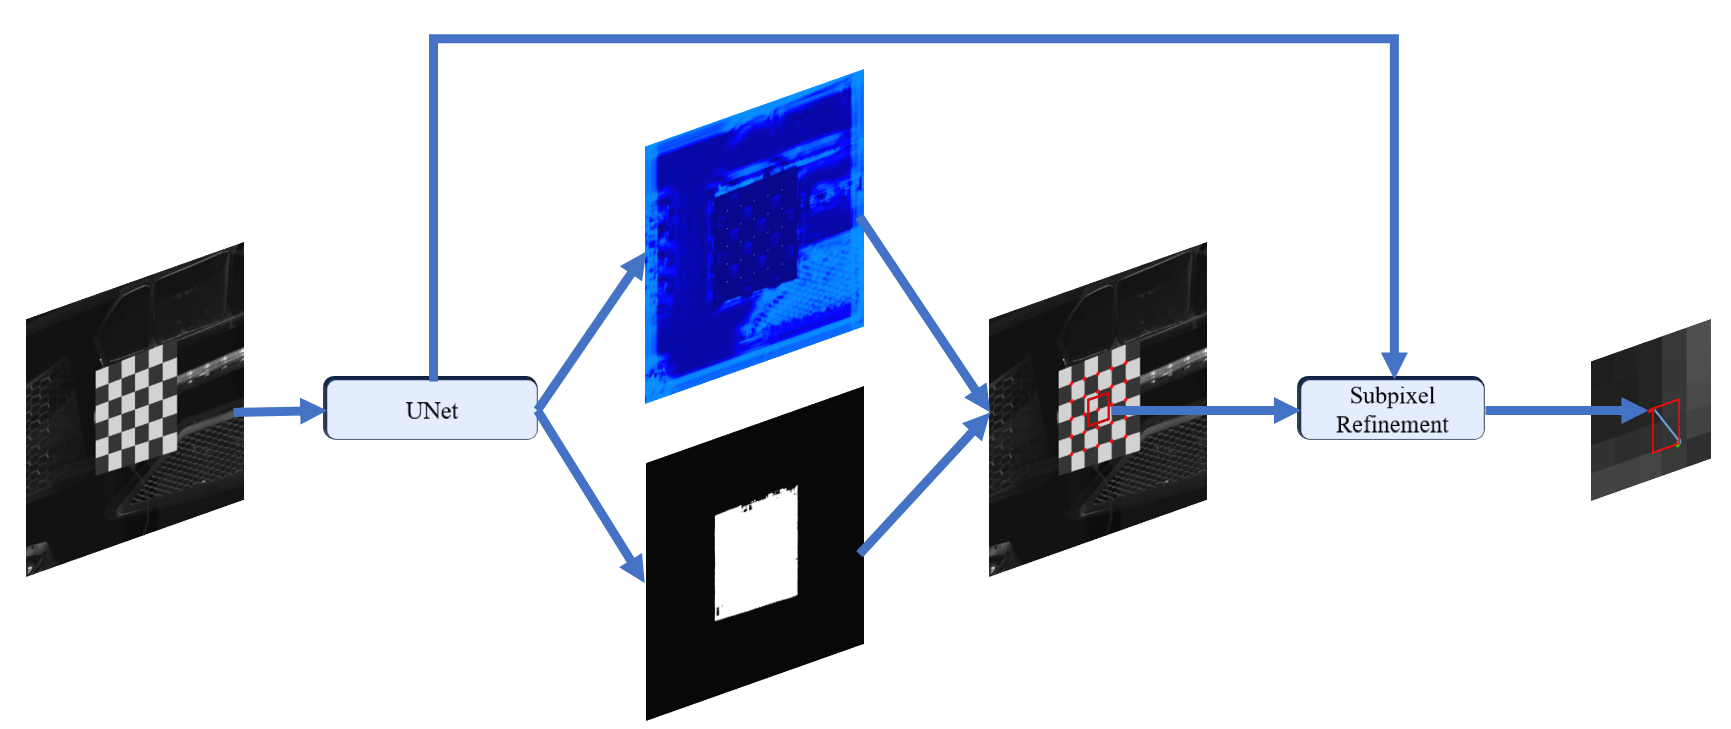
\includegraphics[width=0.8\textwidth]{images/3.png}
\caption{System framework: road sign detection and recognition module coupled with SLAM backend for semantic loop closure.}
\label{fig:framework}
\end{figure}


\section{Related Work}

Existing approaches to visual loop closure and road sign-based localization can be broadly categorized into three areas: appearance-based loop closure detection, road sign detection and recognition, and metric pose estimation from planar targets.

\subsection{Visual Loop Closure Detection}

Loop closure detection has been extensively studied in the visual SLAM literature.
Early approaches relied on bag-of-visual-words (BoW) models~\cite{Harris1988}, which
quantize local image features into a visual vocabulary and use term frequency-inverse
document frequency (TF-IDF) scoring to efficiently retrieve candidate matches from a
database of keyframes. Systems such as ORB-SLAM~\cite{Haralick1992} demonstrated
the effectiveness of BoW-based loop closure in real-time monocular SLAM, achieving
reliable drift correction in indoor and structured outdoor environments.

A fundamental limitation of these feature-based approaches, however, is their
sensitivity to changes in environmental appearance. Under varying illumination,
weather conditions, or seasonal changes, the local features extracted from the same
physical location can differ dramatically, causing BoW-based retrieval to fail.
Researchers have explored several directions to improve appearance robustness,
including the use of learned global descriptors~\cite{VanDeWeijer2006} such as
NetVLAD, which trains a convolutional neural network to produce viewpoint- and
illumination-invariant place descriptors, and sequence-based matching techniques
that exploit temporal consistency to filter unreliable matches.

Object-level SLAM and semantic loop closure represent a more recent paradigm.
Instead of matching low-level features, these methods detect and associate semantic
objects---such as buildings, signs, or landmarks---as loop closure candidates.
Cieslewski et al.~\cite{bennett2014chess} proposed data-efficient decentralized
visual SLAM using object-level data association, while Barbosa et al.~\cite{ocamcalib2006}
demonstrated fiducial marker-based localization for GPS-denied environments.
These approaches are inherently more robust to appearance variation because
semantic object detectors can recognize their targets under significant changes in
viewpoint and lighting.

Road sign detection and recognition has been a active research topic in autonomous
driving. Modern detectors based on YOLO and Faster R-CNN achieve high accuracy
on standard traffic sign benchmarks, and recent works have extended these methods
to handle challenging conditions such as low illumination and motion blur.
However, most existing works treat road sign detection as a standalone perception
task rather than integrating it into the SLAM loop closure pipeline.

Our method differs from prior work by explicitly coupling road sign detection with
the SLAM backend for appearance-robust loop closure. Unlike general object-level
SLAM approaches that rely on arbitrary objects, we exploit the engineered properties
of road signs---standardized appearance, retroreflective materials, and fixed
positions---to achieve reliable re-identification under the exact conditions (fog,
nighttime, rain) that defeat conventional BoW-based methods. Furthermore, we
extend beyond detection to full metric pose estimation by combining looming depth
recovery with feature matching and geometric verification.

\subsection{Metric Pose Estimation from Planar Targets}

Estimating the 6-DoF pose between camera and a known planar target is a classical
problem in computer vision with applications in augmented reality, robot navigation,
and visual SLAM. Given a set of 2D-3D correspondences between image points and
known points on a planar surface, the homography matrix $\mathbf{H}$ can be computed
and decomposed to recover the relative rotation $\mathbf{R}$ and translation $\mathbf{t}$~\cite{Duda2018}.
This approach is widely used for fiducial marker tracking and planar object detection.

A fundamental challenge for monocular pose estimation is scale ambiguity. Without
prior knowledge of the target's physical size or an external metric reference, the
translation recovered from homography decomposition is only up to an unknown
scale factor. This limitation is particularly problematic for loop closure, where the
correct metric scale is essential for meaningful pose graph optimization.

Several strategies have been developed to resolve this scale ambiguity. In RGB-D
systems, the depth channel directly provides metric scale, but commodity depth
sensors have limited effective range (typically 0.6--6~m for stereo-based sensors),
making them unsuitable for distant targets. Stereo visual SLAM systems recover
scale through fixed baseline triangulation, but require sufficient texture and baseline
width. Monocular systems can recover scale through fusion with inertial sensors
or by leveraging known object dimensions as geometric priors.

The looming effect offers an alternative approach to metric depth recovery from
monocular video. As a camera approaches a planar surface, the apparent expansion
of the target in the image plane is directly related to the camera's forward motion
and the absolute depth of the target. By combining the observed expansion ratio
with the inter-frame displacement obtained from visual odometry, the absolute
depth $Z$ can be computed independently of scene texture. This principle has been
applied in aircraft landing guidance and vehicle collision avoidance, but its potential
for metric pose recovery in visual SLAM loop closure remains underexplored.

Deep feature matching has also advanced significantly in recent years. Detector-free
methods such as LoFTR~\cite{opencv_checkerboard} establish dense correspondences
between image pairs using Transformer-based architectures, outperforming traditional
handcrafted features in low-texture and repetitive-pattern scenarios. When combined
with robust estimation techniques such as RANSAC, these correspondences enable
accurate homography computation even under challenging imaging conditions.

Our approach integrates these techniques into a complete metric pose estimation
pipeline for road sign-based loop closure. We leverage the looming effect to recover
the absolute depth of the road sign from temporal monocular observations, inject
this metric scale into the homography decomposition to resolve translation ambiguity,
and employ LoFTR matching with RANSAC to compute the homography robustly
across traversals under varying weather and lighting conditions.



\section{Method}

We present a complete road sign-based loop closure and metric pose estimation system.
The overall pipeline consists of four stages: (1) looming-based absolute depth recovery
from temporal monocular observations; (2) road sign boundary extraction and inter-sequence
feature matching; (3) homography decomposition with metric scale injection for 6-DoF
relative pose estimation; and (4) 3D geometric verification using the road sign's structural
properties. Figure~\ref{fig:pipeline} illustrates the complete system architecture.

\begin{figure}[htbp]
    \centering
    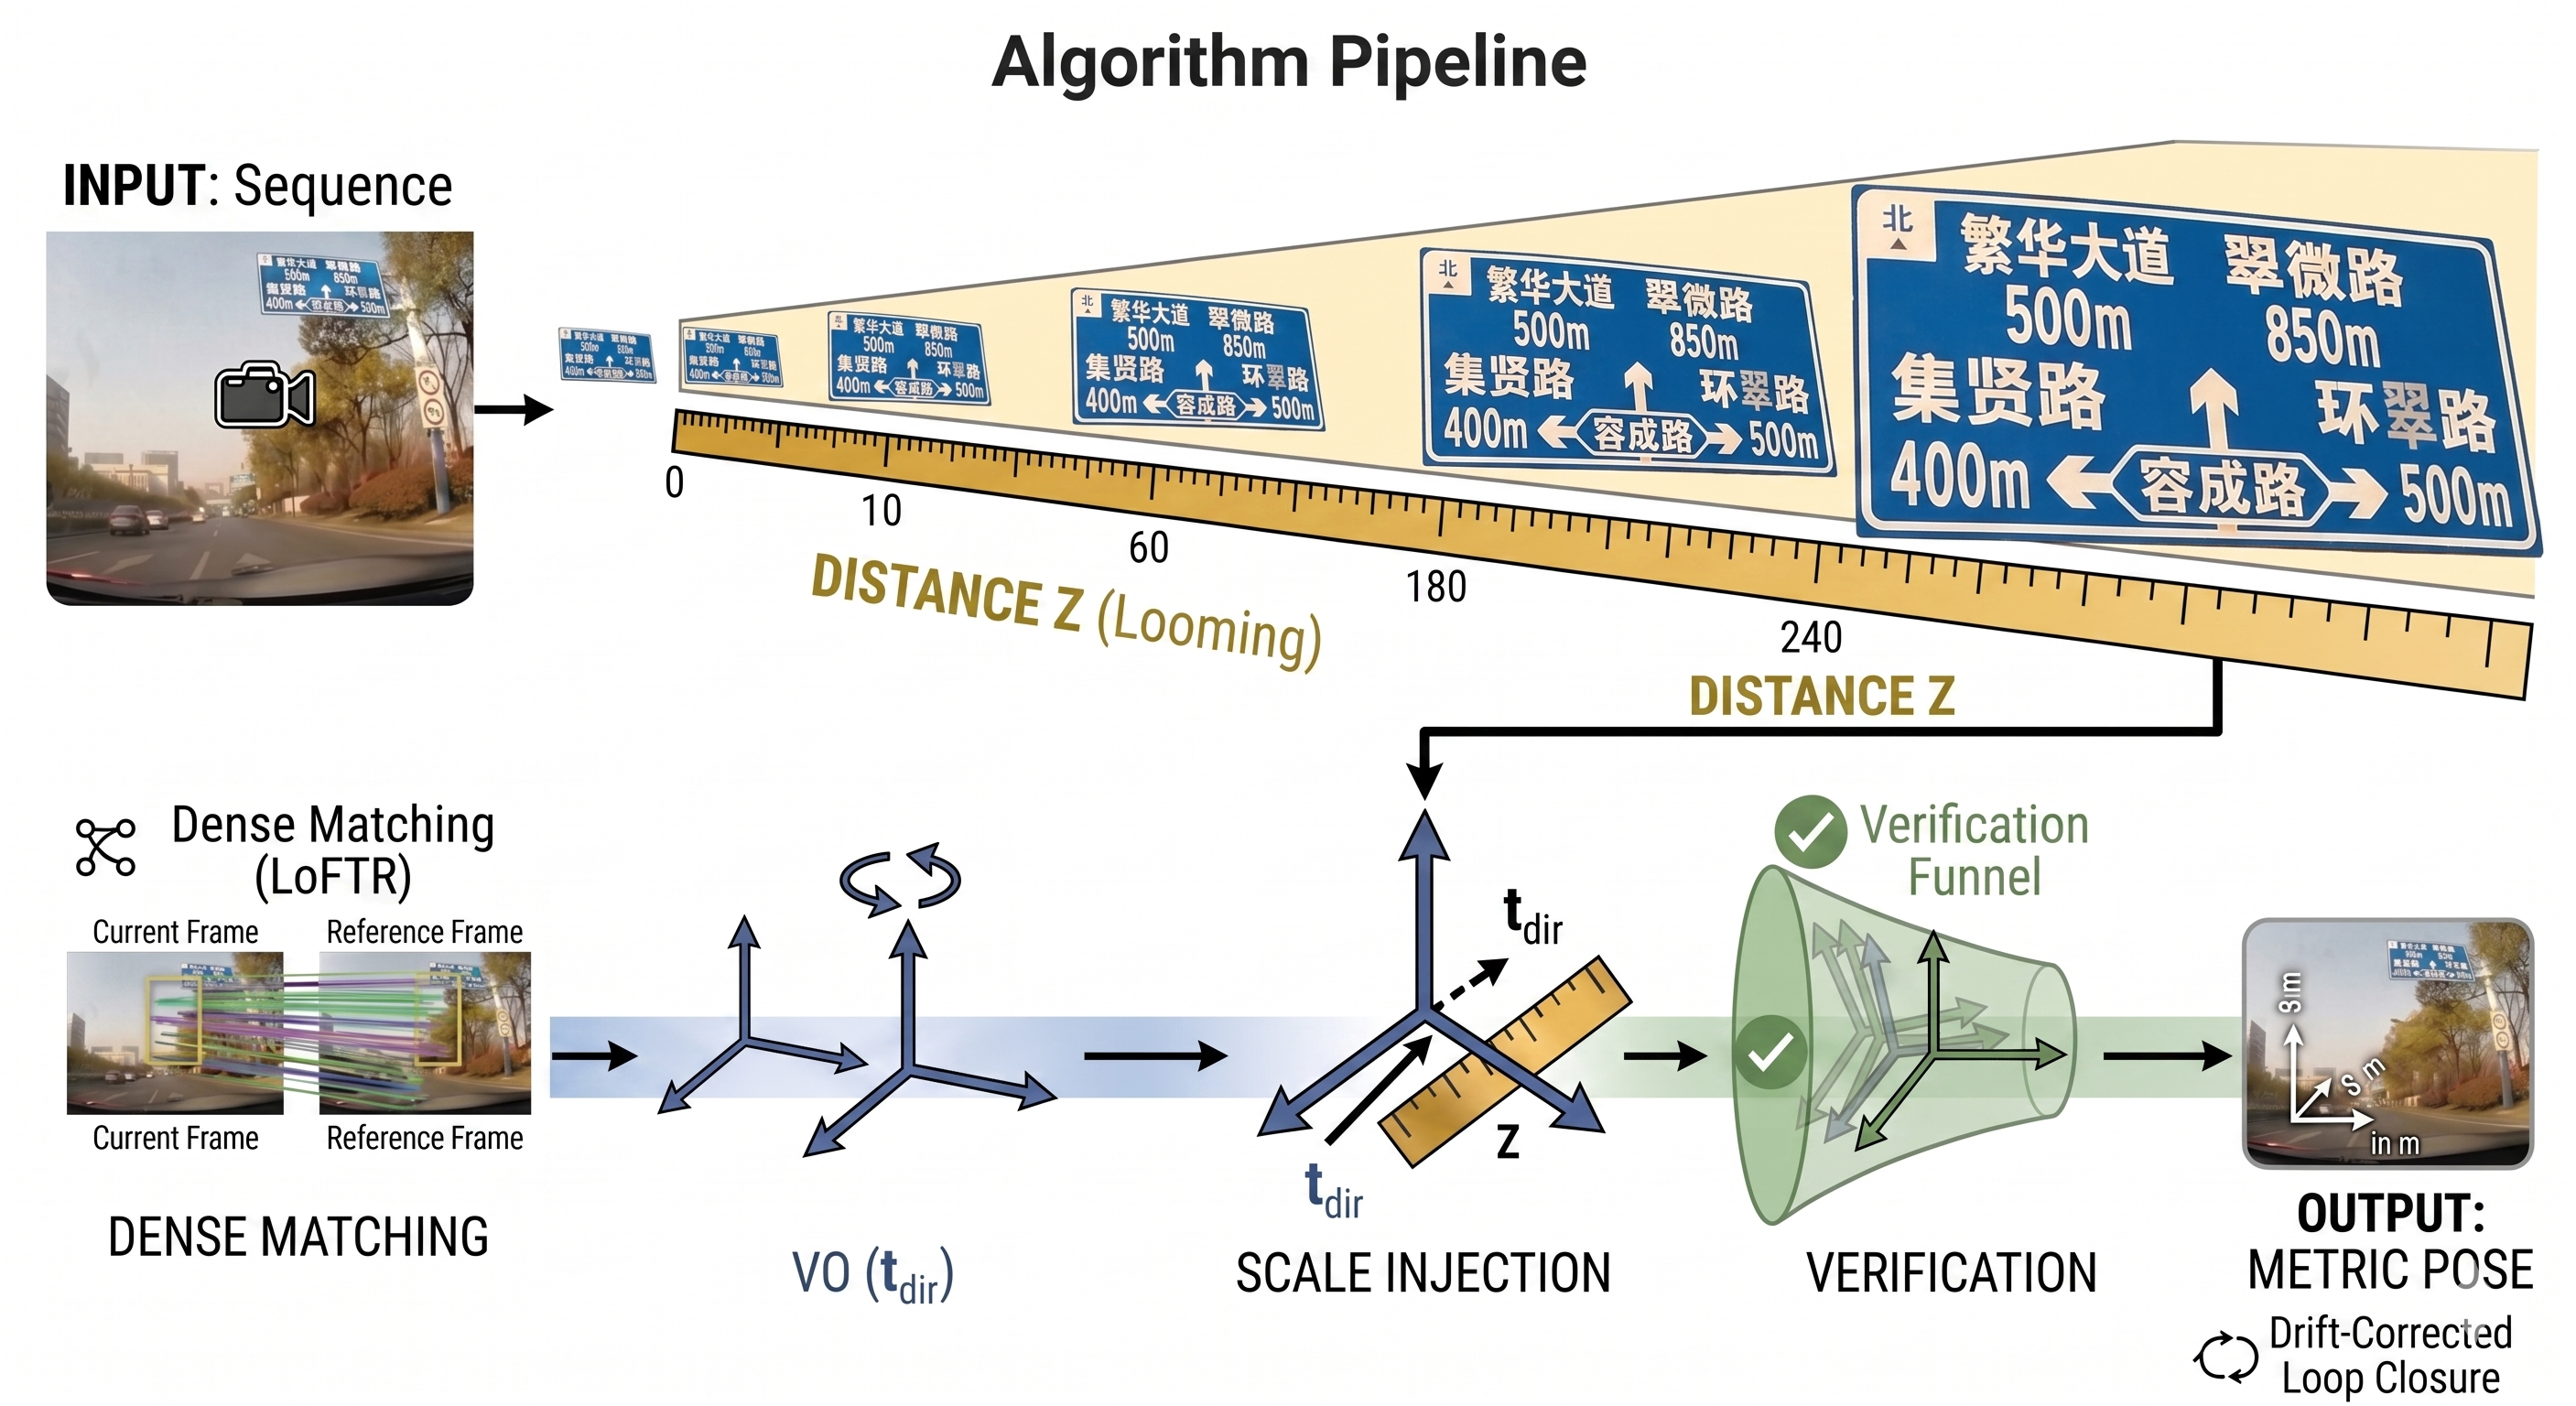
\includegraphics[width=0.8\textwidth]{images/2.png}
    \caption{Proposed road sign-based loop closure and pose estimation pipeline.}
    \label{fig:pipeline}
\end{figure}

\subsection{Looming-based Absolute Depth Recovery}

The first stage recovers the metric depth of the road sign from monocular video
using the looming effect. As the vehicle approaches a planar road sign, the apparent
size of the sign in the image plane expands. By measuring this expansion across
consecutive frames and combining it with the inter-frame camera displacement
obtained from visual odometry, we can compute the absolute depth without any
prior knowledge of the sign's physical dimensions.

Let $\mathbf{P}_{\text{near}} = (u_{\text{near}}, v_{\text{near}})$ and
$\mathbf{P}_{\text{far}} = (u_{\text{far}}, v_{\text{far}})$ denote the center
pixel coordinates of the road sign in two frames separated by a known baseline.
The relative camera motion $\mathbf{R}_{12}$ and $\mathbf{t}_{12}$ between these
frames is obtained from ORB-SLAM3 trajectory. To compensate for rotation, we
derotate the center point from the far frame using the homography induced by
the rotation:

\begin{equation}
\mathbf{P}_{\text{far}}^{\text{derot}} = \pi\left( \mathbf{K} \mathbf{R}_{12}^T \mathbf{K}^{-1} \tilde{\mathbf{P}}_{\text{far}} \right)
\end{equation}

where $\tilde{\mathbf{P}}$ denotes homogeneous coordinates, $\mathbf{K}$ is the
camera intrinsic matrix, and $\pi([X,Y,Z]^T) = [X/Z, Y/Z]$ is the perspective
projection function.

The focus of expansion (FOE) is computed from the translation direction:
\begin{equation}
\mathbf{FOE} = \left( f_x \frac{t_x}{t_z} + c_x,\; f_y \frac{t_y}{t_z} + c_y \right)
\end{equation}

The radial distances from the sign center to the FOE in each frame are:
\begin{equation}
r_{\text{near}} = \|\mathbf{P}_{\text{near}} - \mathbf{FOE}\|,\qquad
r_{\text{far}} = \|\mathbf{P}_{\text{far}}^{\text{derot}} - \mathbf{FOE}\|
\end{equation}

The looming expansion $dr = r_{\text{near}} - r_{\text{far}}$ captures the
apparent growth of the sign as the vehicle approaches. The absolute depth is then
derived from the relationship between radial expansion, forward motion, and depth:

\begin{equation}
Z_{\text{loom}} = \frac{r_{\text{near}} \cdot \Delta d}{dr} - \Delta d
\label{eq:looming}
\end{equation}

where $\Delta d = \|\mathbf{t}_{12}\|$ is the magnitude of the forward translation
between the two frames. This formulation recovers the true metric depth without
requiring any knowledge of the target's physical size, using only the temporal
expansion cue and the relative motion from visual odometry.

\subsection{Road Sign Boundary Extraction and Feature Matching}

Once the road sign region is identified (via ROI annotation or detection), we
extract its four physical boundary lines using a line segment detector (LSD)
within the region of interest. The four detected lines correspond to the top,
bottom, left, and right edges of the sign. From these lines, we compute the
four corner intersection points $\{\mathbf{C}_1, \mathbf{C}_2, \mathbf{C}_3,
\mathbf{C}_4\}$ and the center $\mathbf{P}_{\text{center}}$ via pairwise
line intersection followed by diagonal intersection.

For cross-sequence loop closure, we perform deep feature matching between
the current observation and the reference frame stored in the map. We employ
LoFTR (Local Feature TRansformer), a detector-free feature matcher that
establishes dense correspondences between image pairs using Transformer-based
global and local feature fusion. Given two images $I_1$ (current) and $I_2$
(reference), LoFTR produces a set of 2D-2D correspondences:

\begin{equation}
\mathcal{M} = \{( \mathbf{p}_1^{(i)}, \mathbf{p}_2^{(i)} ) \mid i = 1, \dots, N \}
\end{equation}

These correspondences are filtered using RANSAC to compute the homography
matrix $\mathbf{H}$ that relates the planar road sign between the two views:

\begin{equation}
\mathbf{H} = \arg\min_{\mathbf{H}} \sum_{i} \rho\left(
\left\| \mathbf{p}_2^{(i)} - \pi\left(\mathbf{H} \tilde{\mathbf{p}}_1^{(i)}\right) \right\|^2
\right)
\end{equation}

where $\rho(\cdot)$ is the robust Huber loss function. The RANSAC threshold
is set to 3.0 pixels to reject outlier matches.

\subsection{Homography Decomposition and Metric Scale Recovery}

The homography matrix $\mathbf{H}$ is decomposed into the relative rotation
$\mathbf{R}_{12}$, translation direction $\mathbf{n}$, and plane normal
$\mathbf{n}$ using the analytical decomposition method:

\begin{equation}
\{\mathbf{R}_{12}^{(k)}, \mathbf{t}_{12}^{(k)}, \mathbf{n}^{(k)}\}_{k=1}^{K}
= \text{decomposeHomographyMat}(\mathbf{H}, \mathbf{K})
\label{eq:decomp}
\end{equation}

This decomposition yields up to $K = 4$ mathematically valid solutions. The
translation recovered from homography decomposition is inherently up to an
unknown scale factor: $\mathbf{t}_{12} = \mathbf{t}_n \cdot d$, where $d$ is
the orthogonal distance from the camera to the sign plane.

To resolve this scale ambiguity, we inject the metric depth recovered from the
looming computation. Given the sign center pixel $\mathbf{P}_{\text{center}}$ and
its looming depth $Z_{\text{loom}}$, the 3D point in camera coordinates is:

\begin{equation}
\mathbf{X}_{\text{center}} = Z_{\text{loom}} \cdot \mathbf{K}^{-1}
\tilde{\mathbf{P}}_{\text{center}}
\end{equation}

The orthogonal plane distance $d$ is obtained by projecting this 3D point onto
the plane normal $\mathbf{n}$:

\begin{equation}
d = \mathbf{n}^T \mathbf{X}_{\text{center}}
\label{eq:scale_injection}
\end{equation}

The metric translation is then recovered as $\tilde{\mathbf{t}}_{12} =
\mathbf{t}_n \cdot d$, yielding the full metric 6-DoF relative pose
$\{\mathbf{R}_{12}, \tilde{\mathbf{t}}_{12}\}$ between the two traversals.

\subsection{3D Geometric Verification}

To disambiguate the multiple solutions from homography decomposition and to
validate the final pose estimate, we exploit the structural orthogonality
properties inherent to road signs. Road signs contain well-defined horizontal
and vertical strokes (e.g., text, borders), which form orthogonal sets in 3D.

Given the image lines (horizontal strokes $\mathcal{L}_h$ and vertical strokes
$\mathcal{L}_v$) and the candidate plane normal $\mathbf{n}$, we back-project
the 2D line directions onto the sign plane using the camera model and evaluate
their orthogonality:

\begin{equation}
\epsilon_{\text{ortho}} = \frac{1}{|\mathcal{L}_h||\mathcal{L}_v|}
\sum_{l_h \in \mathcal{L}_h} \sum_{l_v \in \mathcal{L}_v}
\left| \mathbf{d}_h^{(l_h)}( \mathbf{n} ) \cdot \mathbf{d}_v^{(l_v)}( \mathbf{n} ) \right|
\label{eq:ortho}
\end{equation}

where $\mathbf{d}_h$ and $\mathbf{d}_v$ are the 3D direction vectors of the
horizontal and vertical strokes projected onto the plane defined by $\mathbf{n}$.
The correct solution is the one that minimizes this orthogonality error, i.e.,
the candidate for which the back-projected horizontal and vertical strokes are
most perpendicular. This physical prior serves as a powerful disambiguation
criterion without requiring any external calibration objects or inertial
measurements.

\begin{equation}
k^* = \arg\min_{k} \epsilon_{\text{ortho}}^{(k)}
\label{eq:best_solution}
\end{equation}

Once the best solution is identified, the final metric relative pose
$\{\mathbf{R}_{12}^*, \tilde{\mathbf{t}}_{12}^*\}$ is obtained by combining the
selected rotation with the looming-injected translation.



\subsection{Dataset}

To ensure robustness across diverse degradation scenarios, we constructed a large-scale dataset from two sources: directly captured chessboard sequences and digitally augmented variants. Ten distinct patterns, differing in size and X-corner count, were recorded under cluttered backgrounds and non-uniform illumination. The captured images featured minimal distortion and controlled noise, while challenging conditions were synthetically generated by introducing radial and tangential distortions, Gaussian noise, and blur, following the protocol in MATE. All images were converted to grayscale and optionally resized to VGA resolution ($1280\times1280$). A random subset of 3{,}000 images was used for training, with the remainder reserved for validation.


To obtain subpixel-level chessboard corner labels, low-noise chessboard images from various scenes are first collected. The corner candidates are extracted using OpenCV’s \textit{findChessboardCorners} function, but we found their precision is limited. Therefore, we use Bouguet’s algorithm~\cite{bouguet2012camera} to perform subpixel refinement on these candidates, and the resulting corner information is used as the ground-truth annotation. This algorithm achieves high accuracy under low-noise conditions; however, when significant interference occurs, the localization of corners becomes unstable and may lead to errors.



\subsection{Loss Function}
The extreme imbalance between corner and non-corner pixels presents a major challenge for effective pixel-wise corner classification. In high-resolution images, the number of true corners is negligible compared with the total number of pixels, leading to an imbalance ratio far greater than those typically encountered in general object detection tasks. A straightforward mean loss over all pixels tends to bias the network toward predicting only non-corner pixels, whereas even a single missed or false detection can substantially impair checkerboard reconstruction.

To address this issue, we employ a multi-component loss function that integrates pixel-wise corner classification, checkerboard region segmentation, and sub-pixel regression, with its design matching our implementation exactly. For corner classification within the heatmap branch, we combine focal loss to alleviate class imbalance and Tversky loss to adaptively penalize misclassification. 

The focal loss with adaptive weighting is defined as
\begin{equation}
    \mathcal{L}_{\text{focal}} = 
    -\alpha_1 \,(1 - p_t)^{\gamma} \,\log(p_t)
\end{equation}
where 
\begin{equation}
    p_t = G_{ij} \, R_{ij} + \left( 1 - G_{ij} \right) \left( 1 - R_{ij} \right)
\end{equation}
Here, $R_{ij} \in [0,1]$ denotes the predicted confidence score at pixel $(i,j)$ , and $G_{ij} \in \{0,1\}$ represents the corresponding ground-truth label.
The parameter $\alpha_1$ controls the balance between positive and negative samples,
and $\gamma$ gradually increases to focus learning on hard examples with lower $p_t$.



The Tversky loss~\cite{salehi2017tversky} is expressed as
\begin{equation}
    \mathcal{L}_{\text{Tversky}} = 
    1 - \frac{\mathrm{TP} + s}
             {\mathrm{TP} + \alpha_2 \cdot \mathrm{FP} + 
              \beta \cdot \mathrm{FN} + s}
\end{equation}
where \( s \) is a small constant added to avoid division by zero and improve numerical stability.
True Positives (TP) measure the overlap between the predicted region \( R_{ij} \) and the ground truth \( G_{ij} \);
False Positives (FP) correspond to regions predicted by \( R_{ij} \) but not present in \( G_{ij} \);
and False Negatives (FN) correspond to ground-truth regions \( G_{ij} \) that are missed by the prediction \( R_{ij} \).
The parameters \( \alpha_2 \) and \( \beta \) control the relative weighting between FP and FN, respectively.


The combined corner heatmap loss is
\begin{equation}
    \mathcal{L}_1 = \omega_{1} \, \mathcal{L}_{\text{Tversky}} 
                  + \omega_{2} \, \mathcal{L}_{\text{focal}}
\end{equation}

\noindent
In our experiments, we set $\omega_{1} = 0.7$ and $\omega_{2} = 0.3$.



For the Mask Decoder, we employ a combination of binary cross-entropy and Dice losses.
Let \( M_{ij} \in [0,1] \) be the predicted probability of the board mask at pixel \((i,j)\),
and \( G^{M}_{ij} \in \{0,1\} \) the corresponding ground-truth mask value.

The board region loss is defined as
\begin{equation}
    \mathcal{L}_2 = \lambda \, \mathcal{L}_{\text{BCE}} (M, G^{M}) 
    + (1 - \lambda) \, \mathcal{L}_{\text{Dice}} (M, G^{M})
\end{equation}
with \(\lambda = 0.5\).


For regression of sub-pixel corner coordinates, we employ a keypoint coordinate regression loss based on nearest-neighbor matching. Specifically, each corner $(x_i, y_i)$ is assigned to its nearest ground-truth counterpart $(\hat{x}_i, \hat{y}_i)$ in Euclidean space, and the regression error is computed using the L1 distance:
\begin{equation}
    \mathcal{L}_3 = \frac{1}{N} \sum_{i=1}^N \left\{\left\lVert x_i + \Delta x_i - \hat{x}_i \right\rVert_1+\left\lVert y_i + \Delta y_i  - \hat{y}_i \right\rVert_1\right\}
\end{equation}
where $N$ denotes the number of matched keypoints.


Finally, the overall loss function is defined as heatmap loss, board loss, and the keypoint coordinate regression loss based on nearest-neighbor matching:
\begin{equation}
    \mathcal{L}_{\text{total}} = \lambda_a \, \mathcal{L}_{1} + \lambda_b \, \mathcal{L}_2 + \lambda_c \, \mathcal{L}_3
\end{equation}

\noindent
In this formulation, $\mathcal{L}_1$ represents the corner heatmap loss (Tversky + Focal), $\mathcal{L}_2$ corresponds to the board region loss (BCE + Dice), and $\mathcal{L}_3$ denotes the nearest-neighbor regression loss for keypoint coordinates. 
The loss weights $\lambda_a$, $\lambda_b$, and $\lambda_c$ are tunable hyperparameters, set to $\lambda_a = 0.3$, $\lambda_b = 0.1$, and $\lambda_c = 0.6$ in our experiments.






\section{Experiments} 

\subsection{Setting}  
The network is trained with back-propagation and an Adam optimizer with weight decay. In our experiments, we set the learning rate to $5 \times 10^{-5}$ and use a weight decay of $1 \times 10^{-5}$. Additionally, a ReduceLROnPlateau learning rate scheduler is employed, with a patience of 10 epochs and a decay factor of $0.5$.The batch size is set to 2 images due to memory constraints associated with high-resolution images, and training is performed for a total of 200 epochs. To initialize the network, we employ the Xavier weight initialization method, ensuring robust convergence. Biases are initialized with the constant $0.1$.

To evaluate the network during training, we use a validation set split from the training data. The validation loss is monitored, and the model checkpoint with the lowest validation loss is saved. This ensures that the final model generalizes well to unseen data.

\subsection{Performance Evaluation}

We conducted a precision benchmark comparing our corner detection method with Zhang’s calibration~\cite{zhang2002flexible} and three recent algorithms~\cite{ma2008robust,geiger2012automatic,wu2020checkerboard}, as well as a baseline version of our model without the Subpixel Refinement Module. All methods were evaluated on stitched checkerboard images after preprocessing. Ground truth coordinates were manually annotated by marking rectangular regions at each corner and extracting centroid positions. Precision was measured as the mean Euclidean distance between predicted and annotated coordinates.

Additionally, to evaluate the sub-pixel precision of each algorithm, we generated synthetic checkerboard samples using the Unity engine. This simulation allowed us to obtain exact corner pixel coordinates for benchmarking. The corner detection precision on these synthetic samples was then assessed, ensuring an accurate evaluation beyond real-world annotated data.

Results (Fig.~\ref{fig:comparison}, Table~\ref{tab:comparison}) show that Zhang’s method~\cite{zhang2002flexible} achieved 96.97\% accuracy with negligible false detections under normal conditions, but in noisy scenes missed 8.76\% of corners and had $1.10$~pixel error, and under occlusion its success rate fell below 38\% without geometric completion (Fig.~\ref{fig:comparison} (a)). The chord-to-point distance accumulation~\cite{ma2008robust} was noise-sensitive, yielding 28.19\% false detections, 71.81\% accuracy, and $0.87$~pixel error (Fig.~\ref{fig:comparison} (b)). The method in~\cite{geiger2012automatic} reached 95.94\% accuracy but systematically missed boundary corners, with 4.06\% false detections and $1.09$~pixel error (Fig.~\ref{fig:comparison} (c)). The approach in~\cite{wu2020checkerboard} suffered structural interference, producing high false detections and up to $1.20$~pixel error (Fig.~\ref{fig:comparison} (d)).In addition, Fig.~\ref{fig:comparison1} provides a detailed comparison of the differences in sub-pixel accuracy across various algorithms.Our algorithm, enhanced with a sub-pixel refinement module, achieved 97.68\% complete detection and a $0.47$~pixel error. Experiments were conducted on an Intel Core i9-12900KF CPU and an NVIDIA RTX 3090 GPU. 


\begin{figure*}[htbp]
\centering
% 第一行
\begin{minipage}{0.19\textwidth}
    \centering
    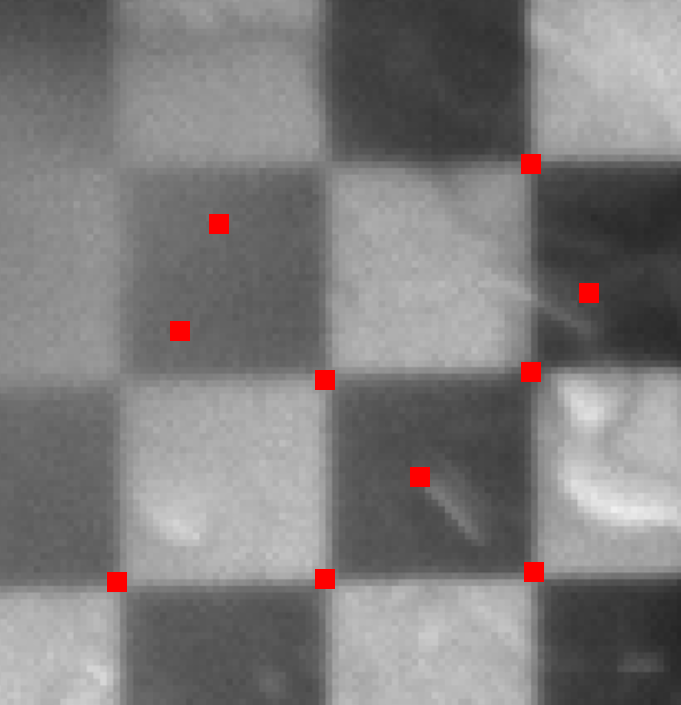
\includegraphics[width=\linewidth]{images/a.png}
\end{minipage}
\begin{minipage}{0.19\textwidth}
    \centering
    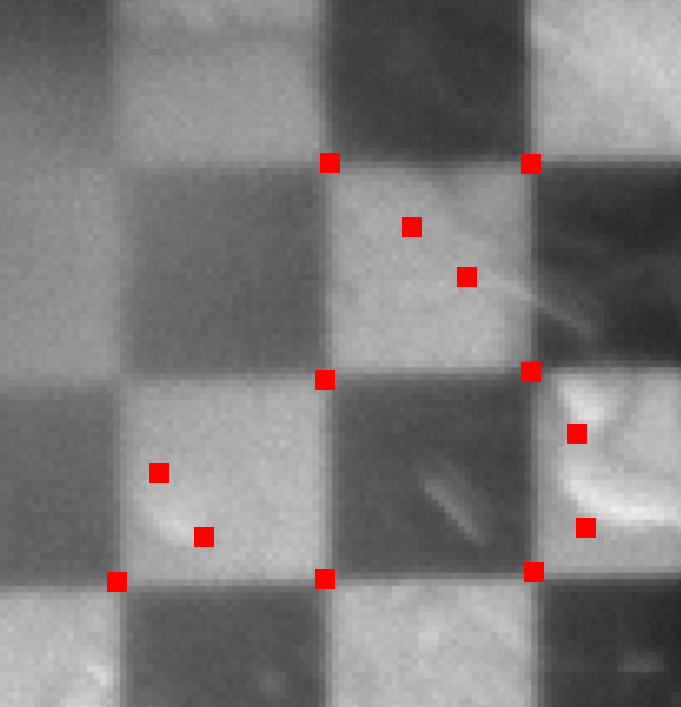
\includegraphics[width=\linewidth]{images/b.png}
\end{minipage}
\begin{minipage}{0.19\textwidth}
    \centering
    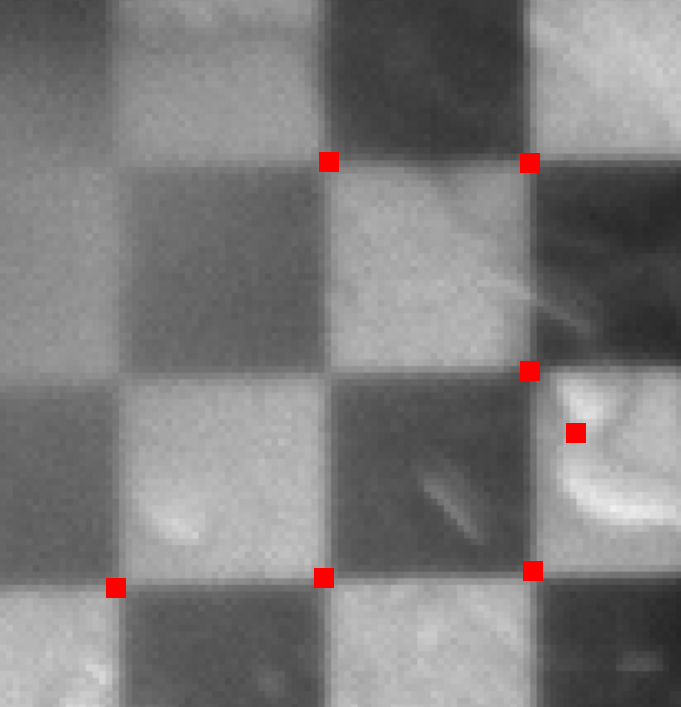
\includegraphics[width=\linewidth]{images/c.png}
\end{minipage}
\begin{minipage}{0.19\textwidth}
    \centering
    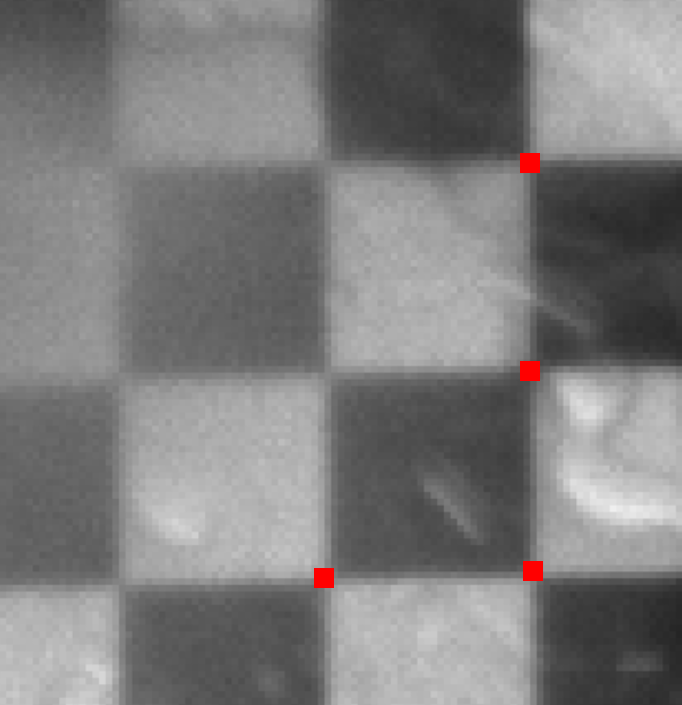
\includegraphics[width=\linewidth]{images/d.png}
\end{minipage}
\begin{minipage}{0.19\textwidth}
    \centering
    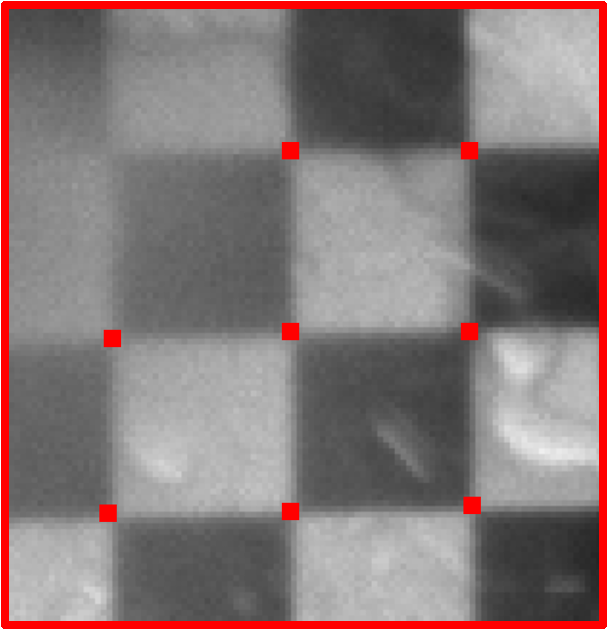
\includegraphics[width=\linewidth]{images/e.png}
\end{minipage}

\vspace{0.5em} % 两行图间距

% 第二行
\begin{minipage}{0.19\textwidth}
    \centering
    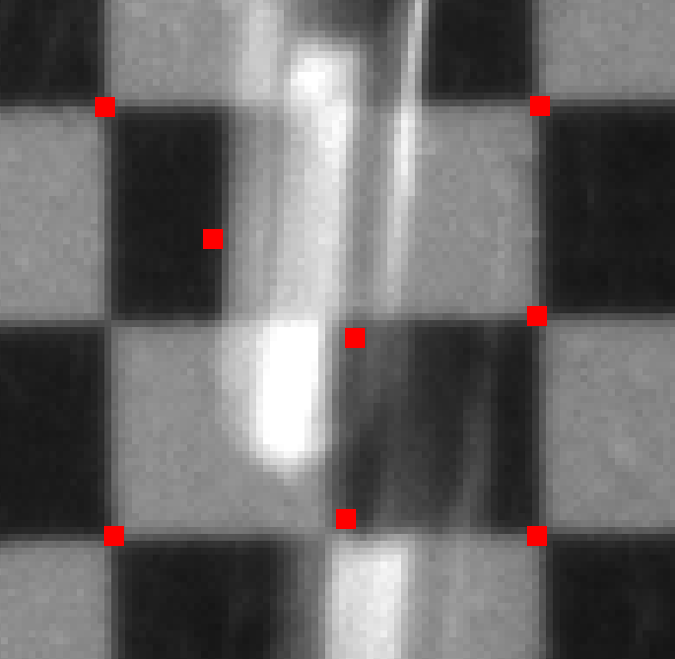
\includegraphics[width=\linewidth]{images/a1.png}
\end{minipage}
\begin{minipage}{0.19\textwidth}
    \centering
    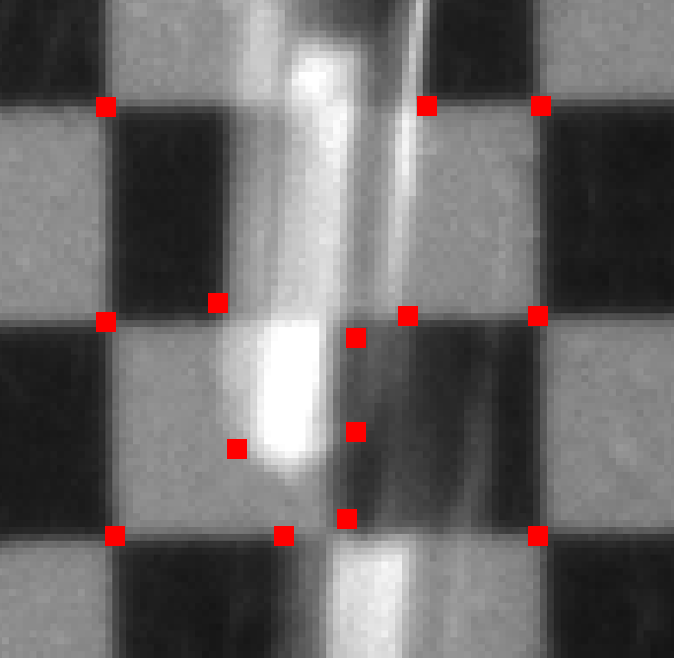
\includegraphics[width=\linewidth]{images/b1.png}
\end{minipage}
\begin{minipage}{0.19\textwidth}
    \centering
    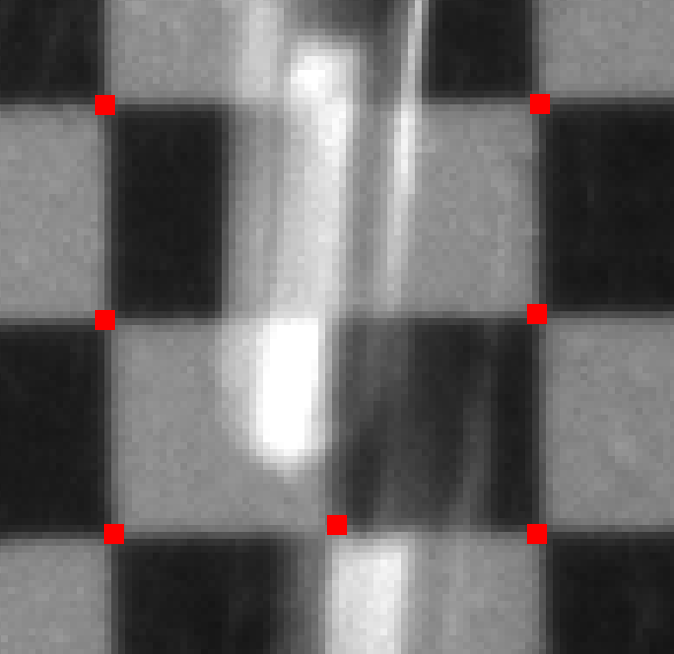
\includegraphics[width=\linewidth]{images/c1.png}
\end{minipage}
\begin{minipage}{0.19\textwidth}
    \centering
    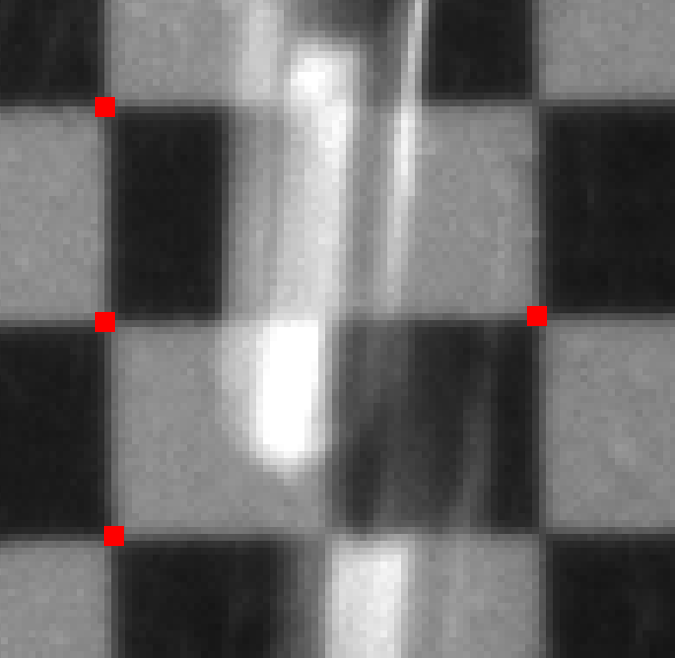
\includegraphics[width=\linewidth]{images/d1.png}
\end{minipage}
\begin{minipage}{0.19\textwidth}
    \centering
    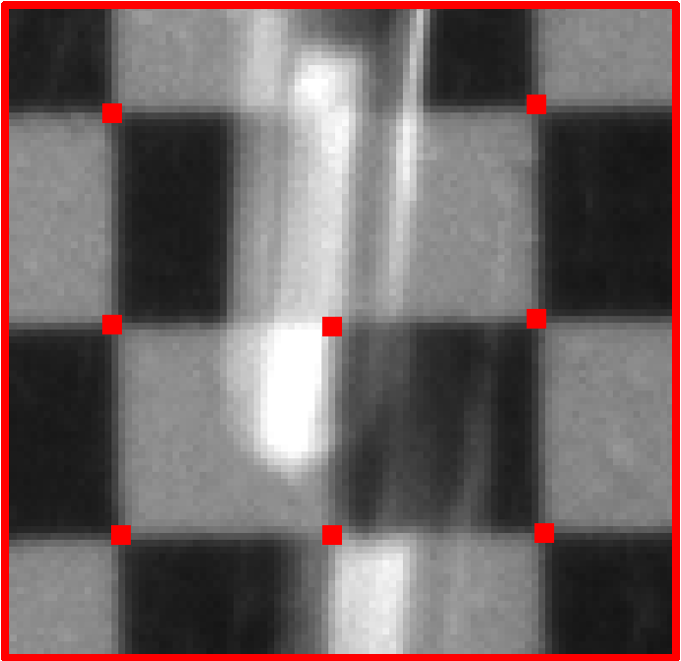
\includegraphics[width=\linewidth]{images/e1.png}
\end{minipage}

\vspace{0.5em} % 两行图间距

% 第二行
\begin{minipage}{0.19\textwidth}
    \centering
    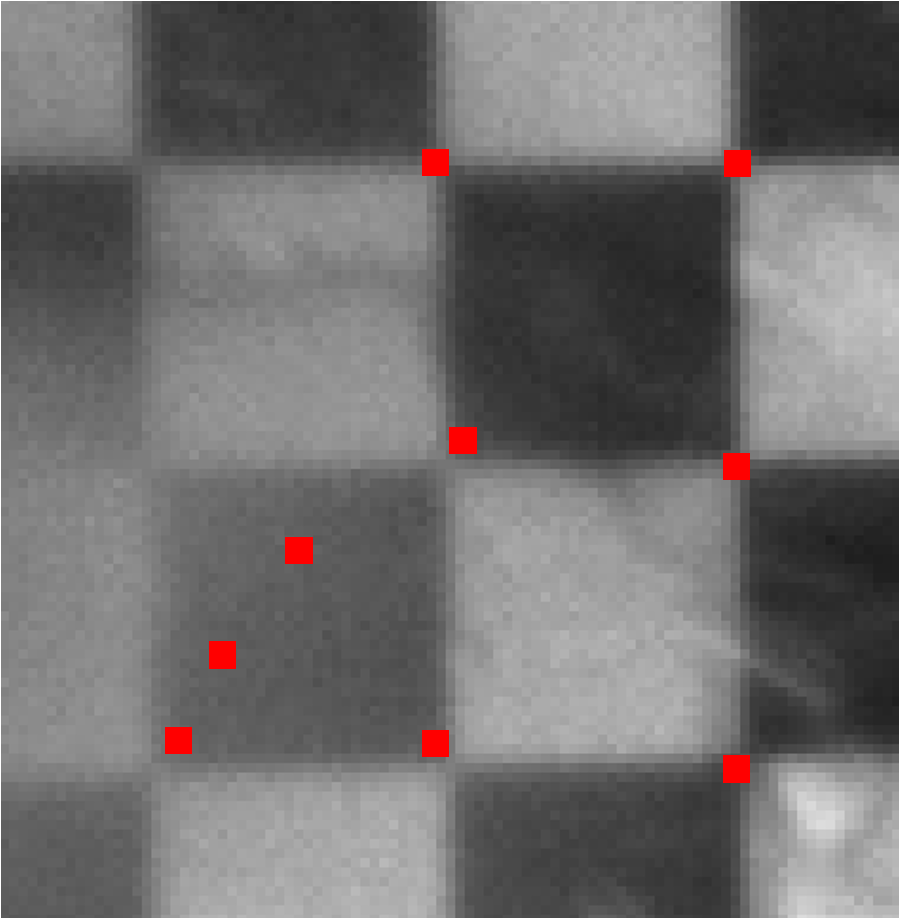
\includegraphics[width=\linewidth]{images/6-1.png}
\end{minipage}
\begin{minipage}{0.19\textwidth}
    \centering
    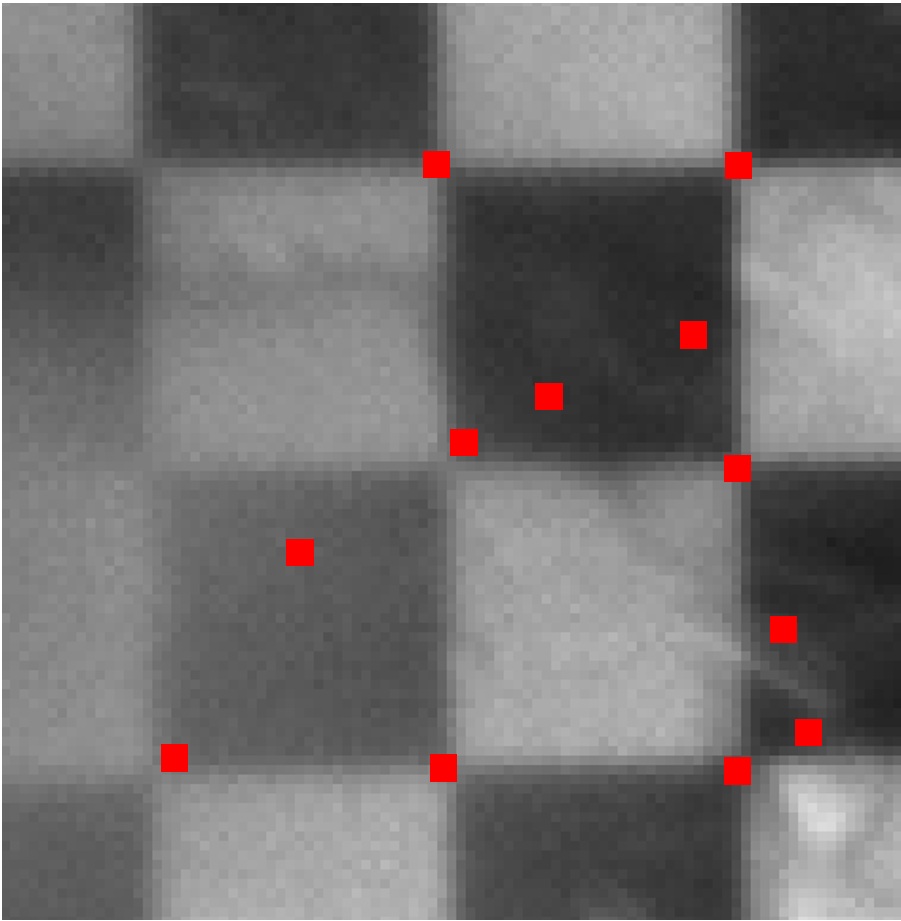
\includegraphics[width=\linewidth]{images/6-2.png}
\end{minipage}
\begin{minipage}{0.19\textwidth}
    \centering
    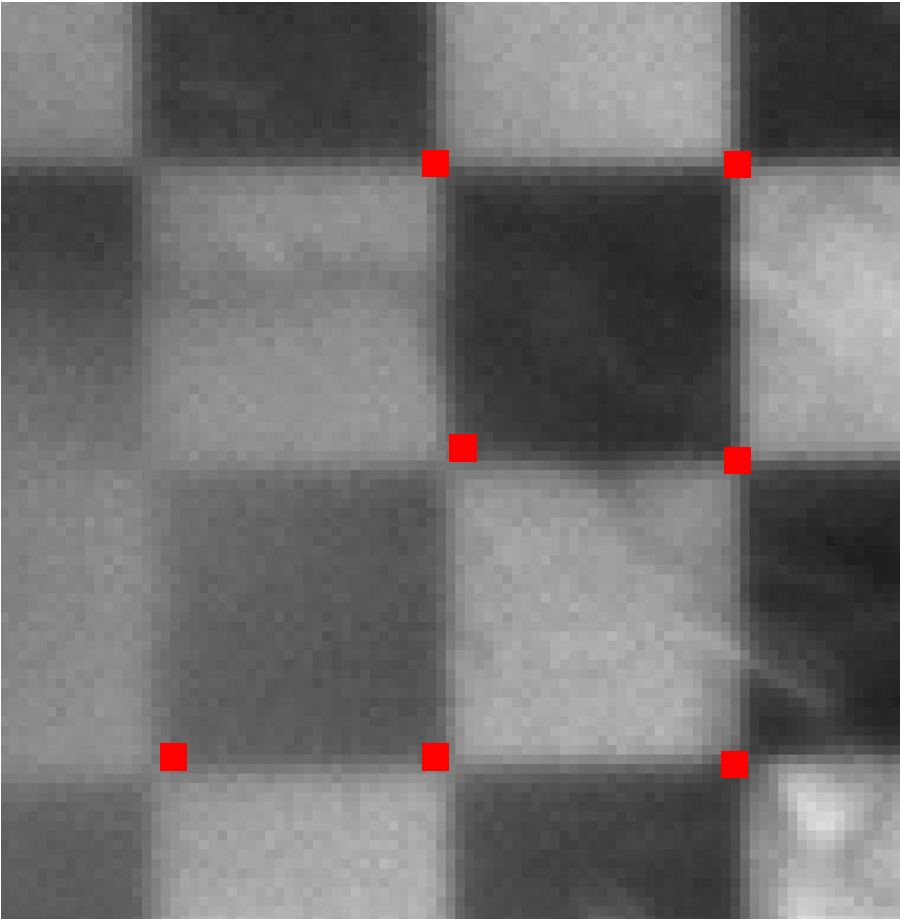
\includegraphics[width=\linewidth]{images/6-3.png}
\end{minipage}
\begin{minipage}{0.19\textwidth}
    \centering
    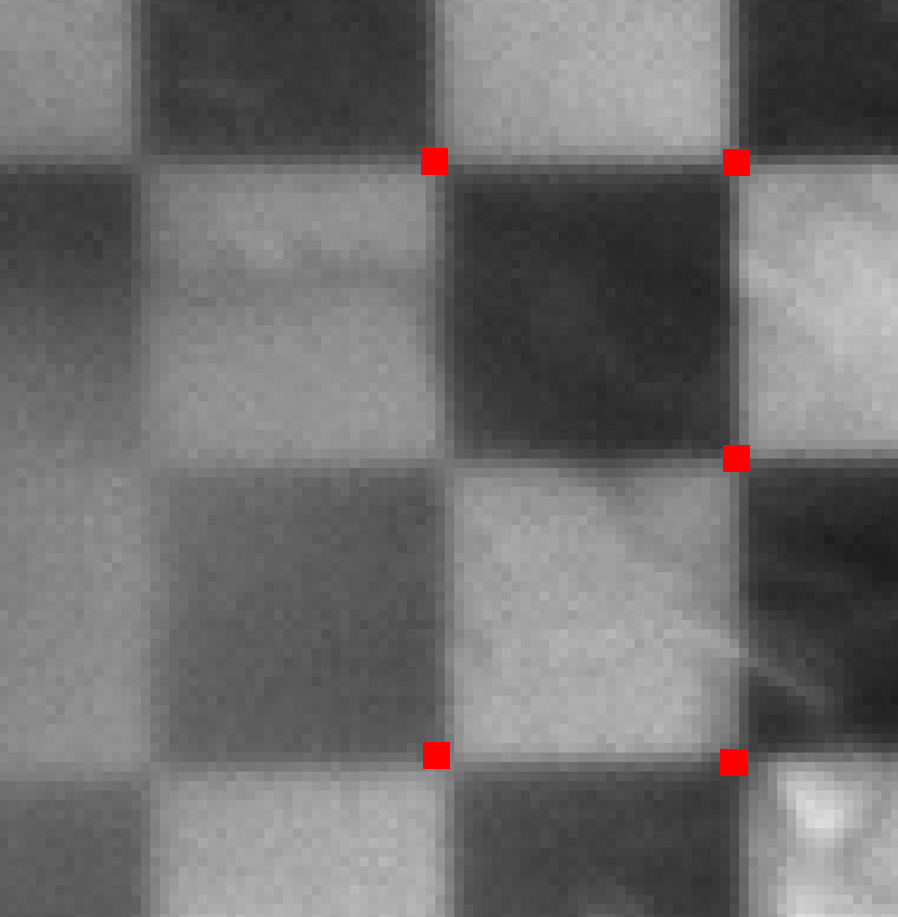
\includegraphics[width=\linewidth]{images/6-4.png}
\end{minipage}
\begin{minipage}{0.19\textwidth}
    \centering
    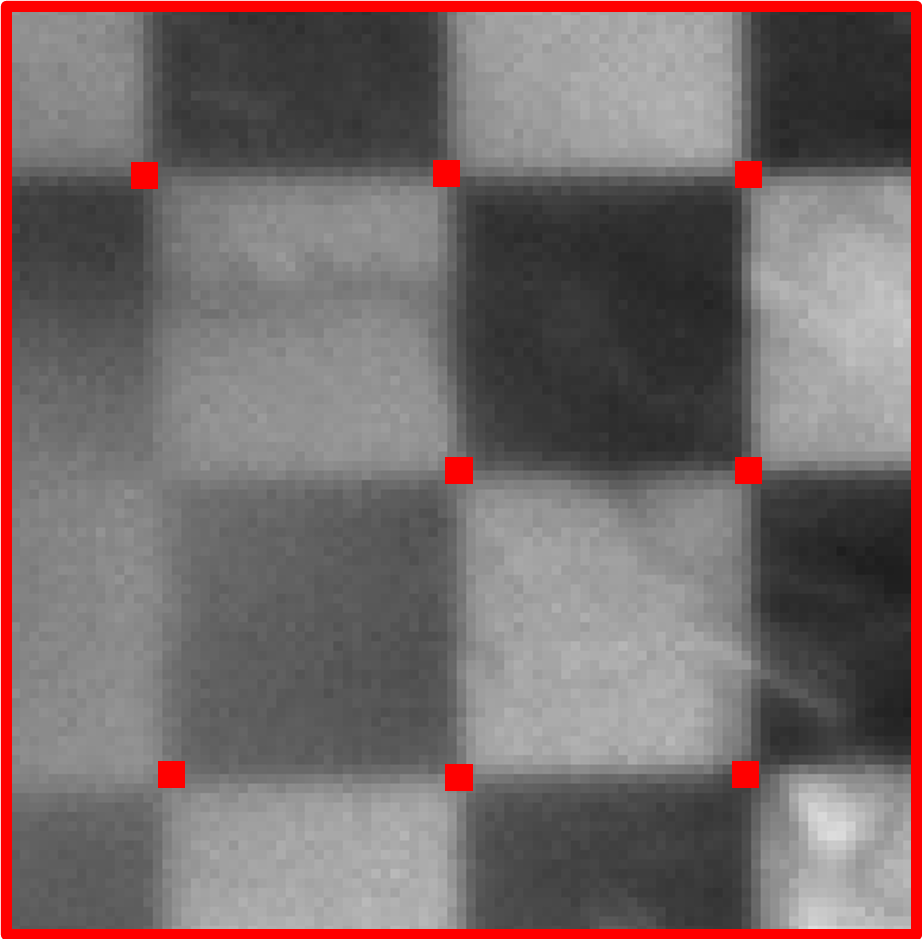
\includegraphics[width=\linewidth]{images/6-5.png}
\end{minipage}

\vspace{0.5em} % 两行图间距

% 第二行
\begin{minipage}{0.19\textwidth}
    \centering
    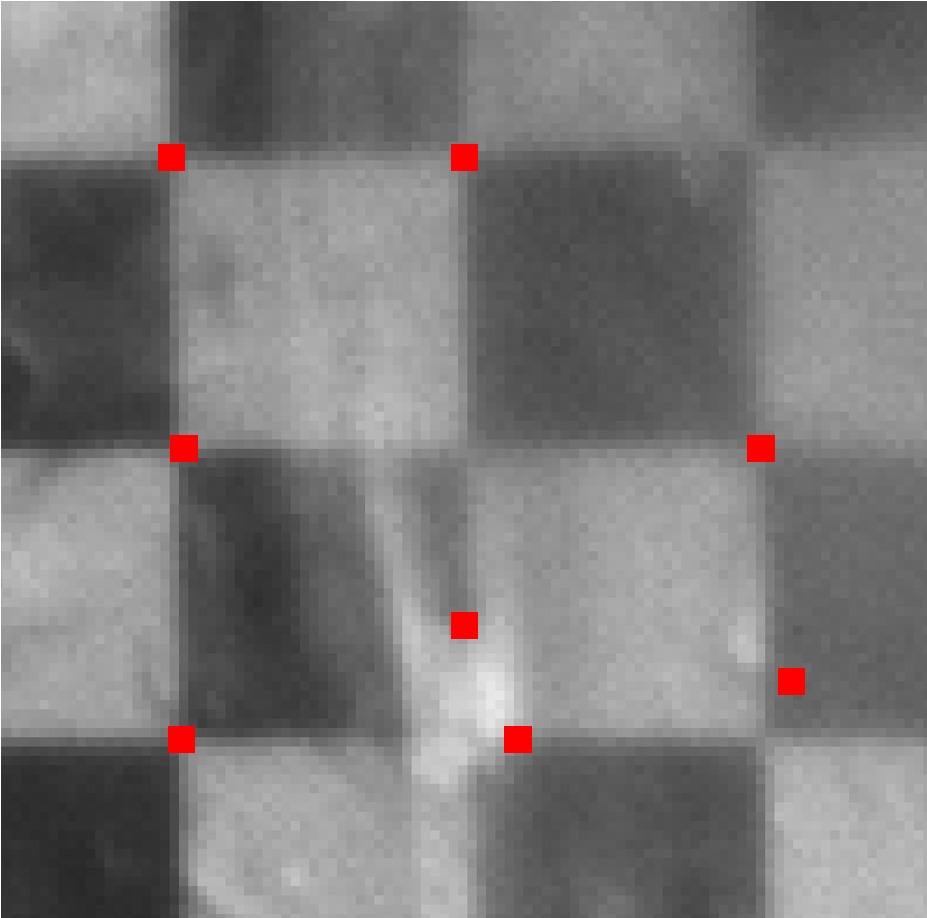
\includegraphics[width=\linewidth]{images/7-1.png}
    \subcaption{(a)}
\end{minipage}
\begin{minipage}{0.19\textwidth}
    \centering
    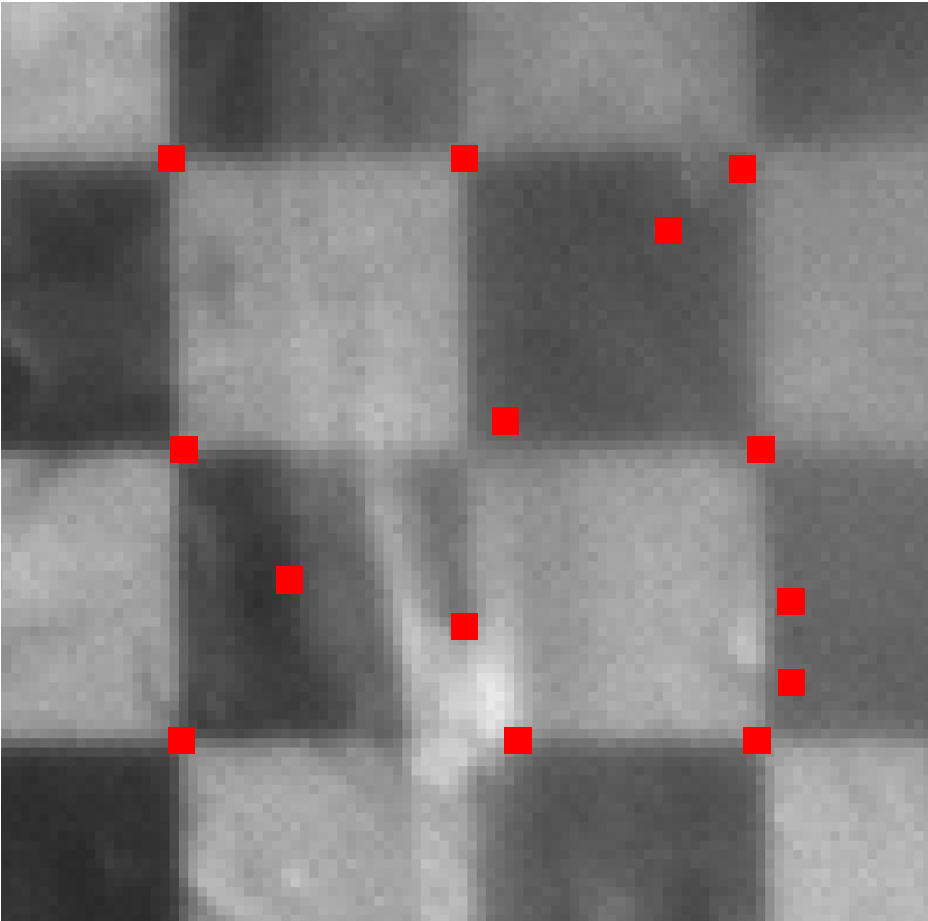
\includegraphics[width=\linewidth]{images/7-2.png}
    \subcaption{(b)}
\end{minipage}
\begin{minipage}{0.19\textwidth}
    \centering
    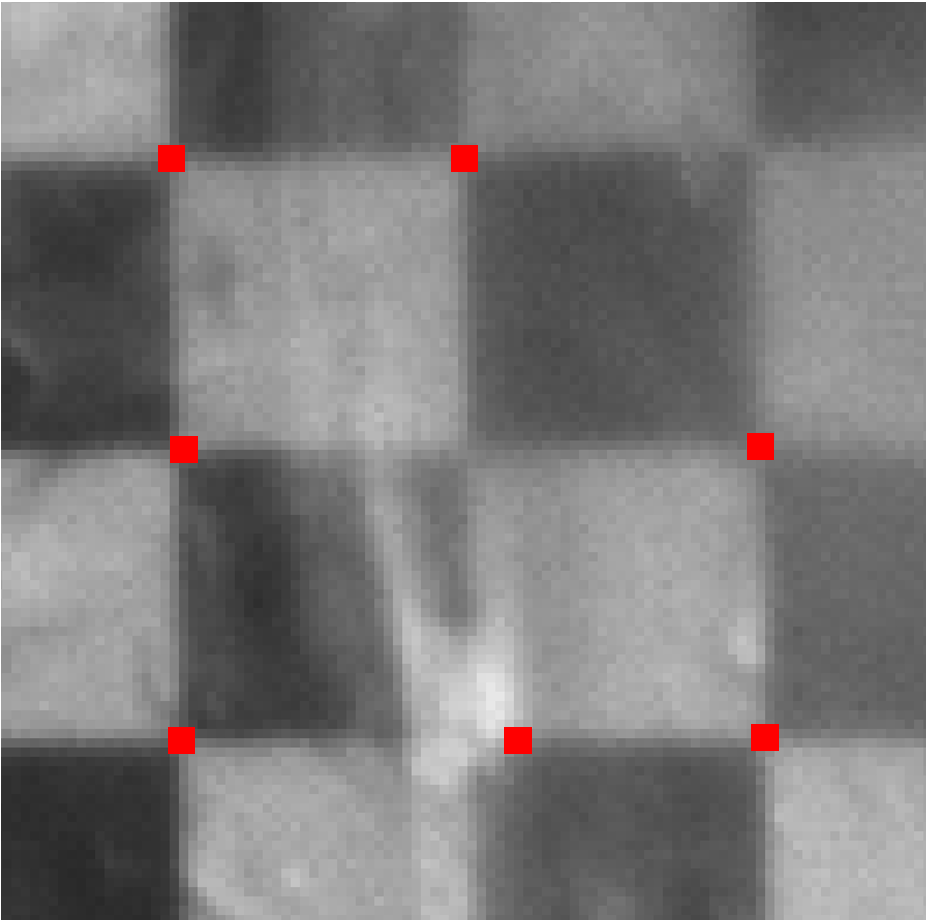
\includegraphics[width=\linewidth]{images/7-3.png}
    \subcaption{(c)}
\end{minipage}
\begin{minipage}{0.19\textwidth}
    \centering
    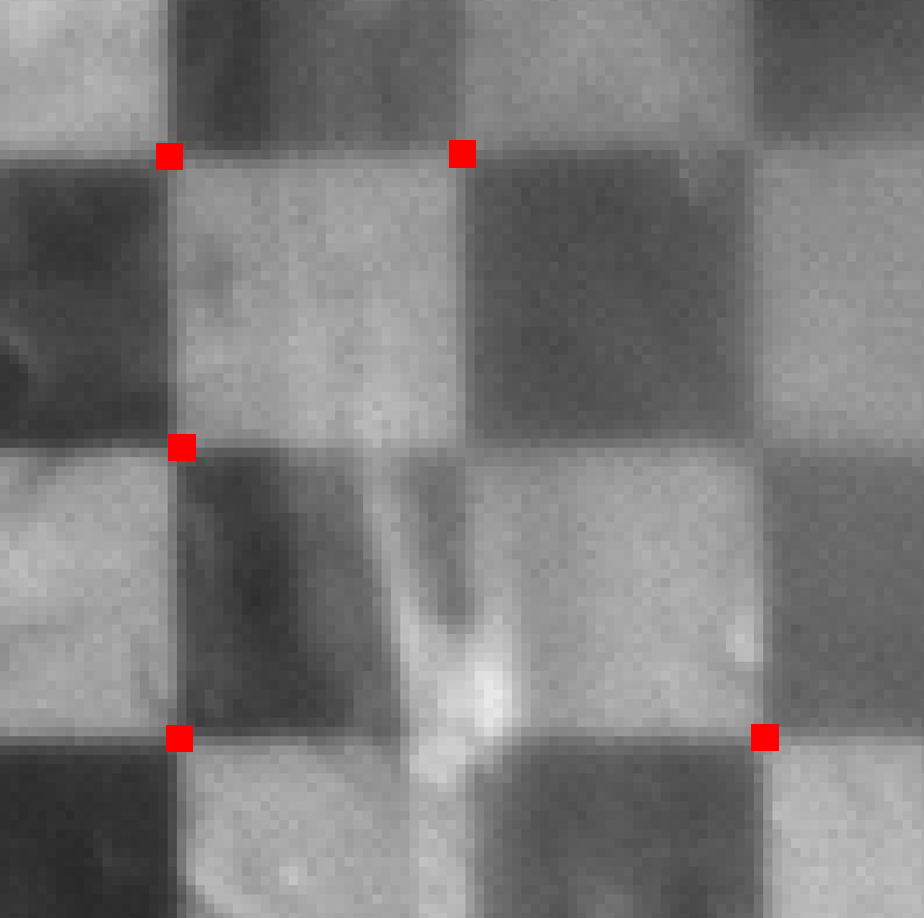
\includegraphics[width=\linewidth]{images/7-4.png}
    \subcaption{(d)}
\end{minipage}
\begin{minipage}{0.19\textwidth}
    \centering
    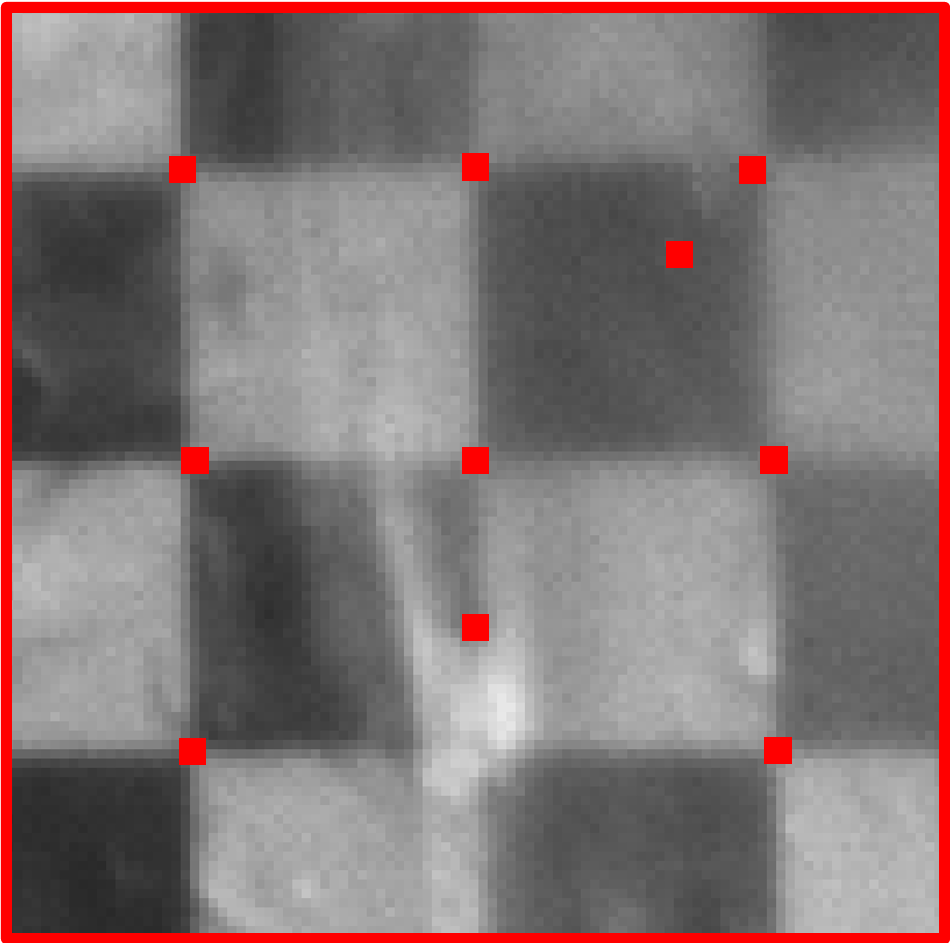
\includegraphics[width=\linewidth]{images/7-5.png}
    \subcaption{(e)}
\end{minipage}

\caption{Summary of issues in corner detection under non-occluded and occluded conditions. 
The red dots depicted in the images represent the identified coordinates of the corners. 
(a) Zhang.~\cite{zhang2002flexible} (b) Awrangjeb.~\cite{ma2008robust}. (c) Geiger.~\cite{geiger2012automatic}. (d) Wu.~\cite{wu2020checkerboard}. (e) Ours.}
\label{fig:comparison}
\end{figure*}

\begin{figure*}[htbp]
\centering
\begin{minipage}{0.20\textwidth}
    \centering
    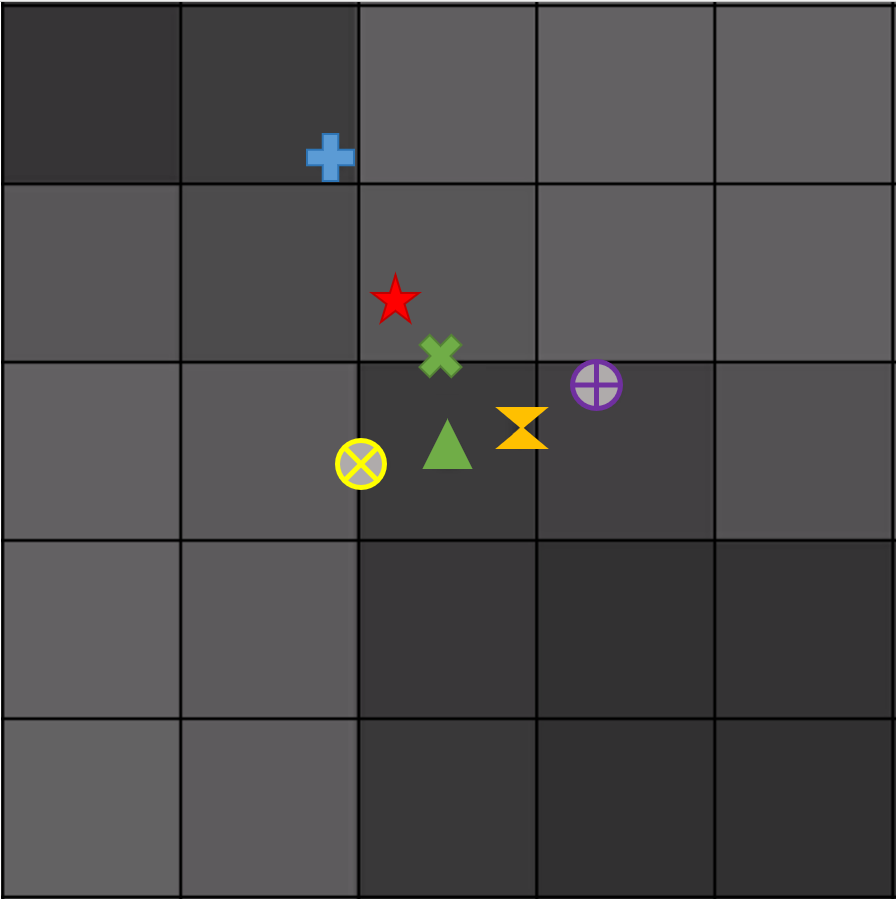
\includegraphics[width=\linewidth,height=1\textwidth]{images/4-1.png}
\end{minipage}
\hspace{0.2em}   % 调整缝隙，单位可用 em, cm, mm
\begin{minipage}{0.20\textwidth}
    \centering
    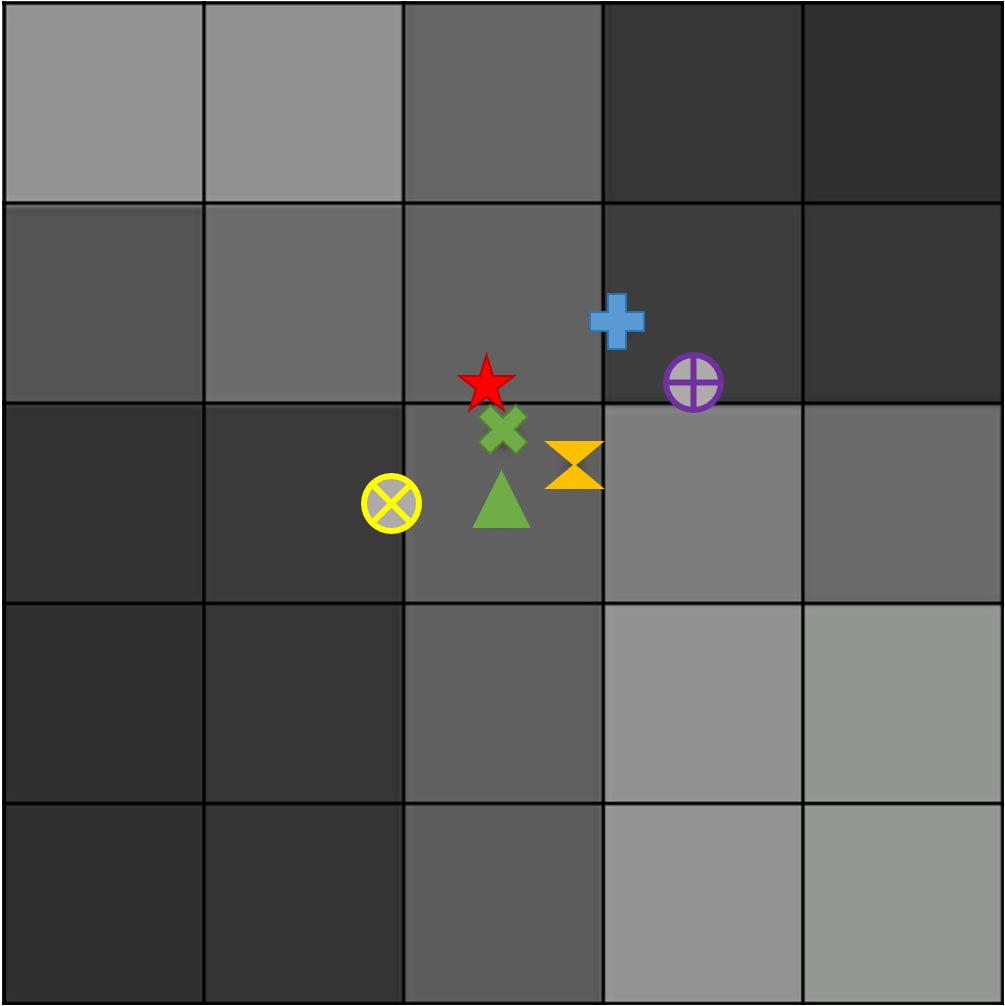
\includegraphics[width=\linewidth,height=1\textwidth]{images/4-2.png}
\end{minipage}
\hspace{0.2em}
\begin{minipage}{0.20\textwidth}
    \centering
    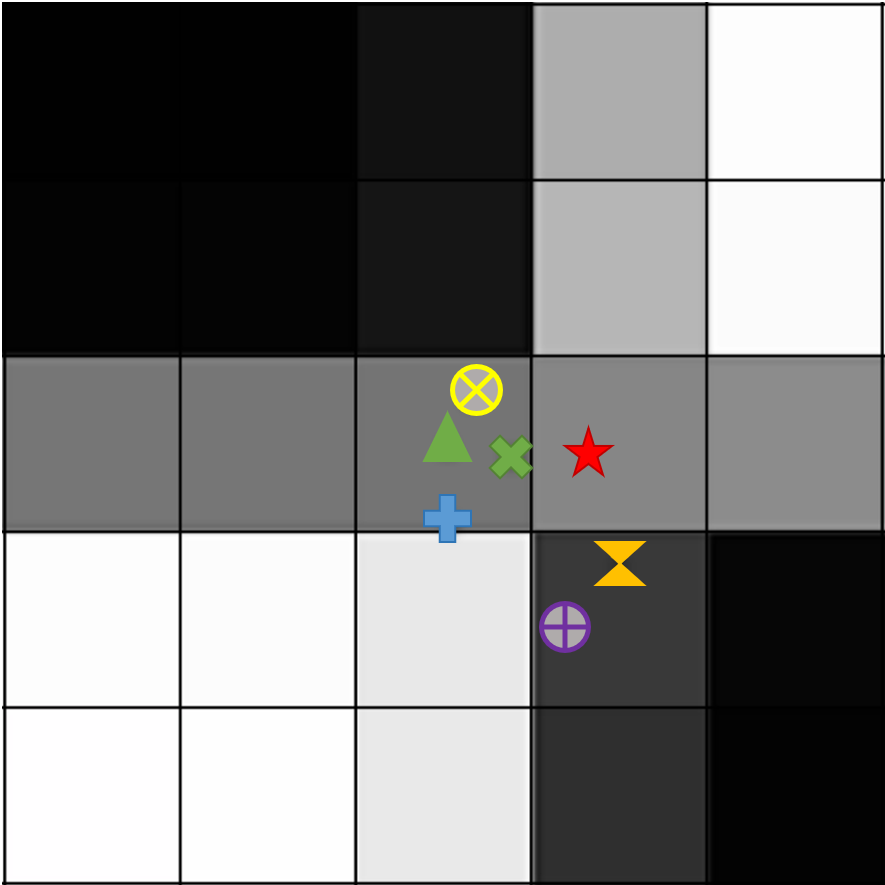
\includegraphics[width=\linewidth,height=1\textwidth]{images/4-3.png}
\end{minipage}
\hspace{0.2em}
\begin{minipage}{0.20\textwidth}
    \centering
    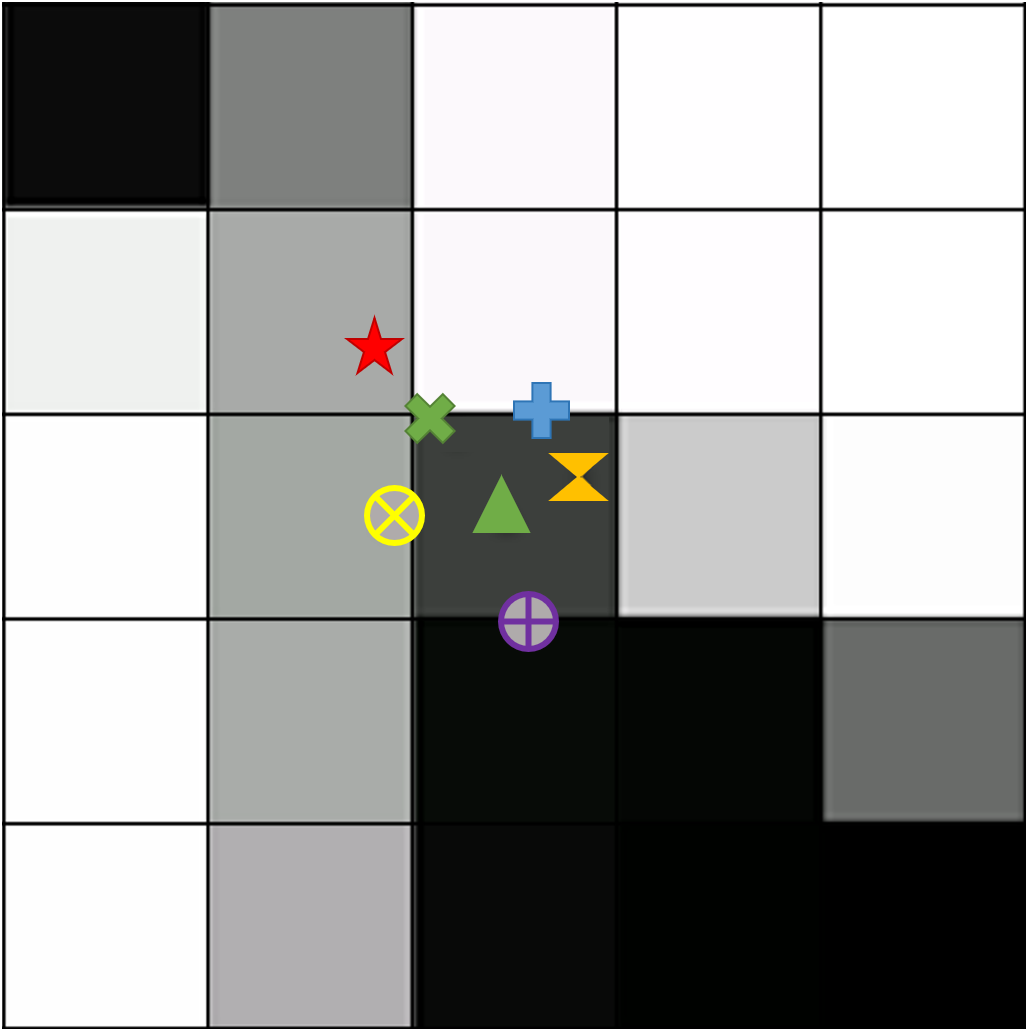
\includegraphics[width=\linewidth,height=1\textwidth]{images/4-4.png}
\end{minipage}
\hspace{0.2em}
\begin{minipage}{0.7\textwidth}
    \centering
    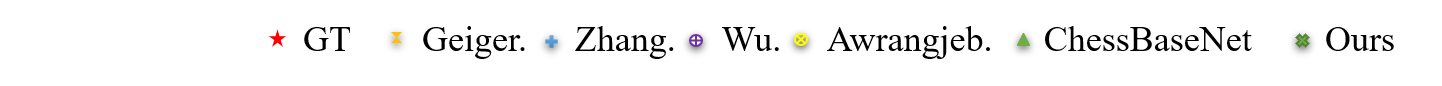
\includegraphics[width=\linewidth,height=0.065\textwidth]{images/4-5.png}
\end{minipage}

\caption{Corner Detection Accuracy Comparison. Each colored block represents a single pixel, and different point shapes indicate distinct corner detection algorithms as illustrated.}
\label{fig:comparison1}
\end{figure*}



\begin{table}[htbp]
\centering
\caption{Comparative analysis of corner detection methods.}
\label{tab:comparison}
\begin{tabular}{lcccc}
\toprule
\hline
\textbf{Algorithm} & \textbf{Precision (\%)} & \textbf{Recall (\%)} & \textbf{Bias (pixel)}  \\
\hline
Zhang.~\cite{zhang2002flexible} & 96.9787 & 91.2398 & 1.0978  \\
Awrangjeb.~\cite{ma2008robust} & 71.8144 & 94.8411 & 0.8693  \\
Geiger.~\cite{geiger2012automatic} & 95.9423 & 73.1123 & 1.0902  \\
Wu.~\cite{wu2020checkerboard} & 93.8793 & 85.6621 & 1.2022  \\
ChessBaseNet & 93.2313 & 93.3161 & 0.7311  \\
Ours & \textbf{97.6775} & \textbf{94.9801} & \textbf{0.4684}  \\
\hline
\bottomrule
\end{tabular}
\end{table}

We additionally conducted a comparative experiment to evaluate the robustness of Bouguet’s algorithm~\cite{bouguet2012camera} under image degradation conditions. In this test, both our Subpixel Refinement Module and Bouguet’s algorithm were provided with the same pixel-level corner coordinates as input. As shown in Fig.~\ref{fig:comparison3}, Bouguet’s algorithm fails to estimate precise corner localization when image quality deteriorates, exhibiting noticeable positional shifts. In contrast, our Subpixel Refinement Module preserves accurate corner positions under the same conditions, demonstrating robustness in detection performance.


\begin{figure*}[htbp]
\centering
\begin{minipage}{0.20\textwidth}
    \centering
    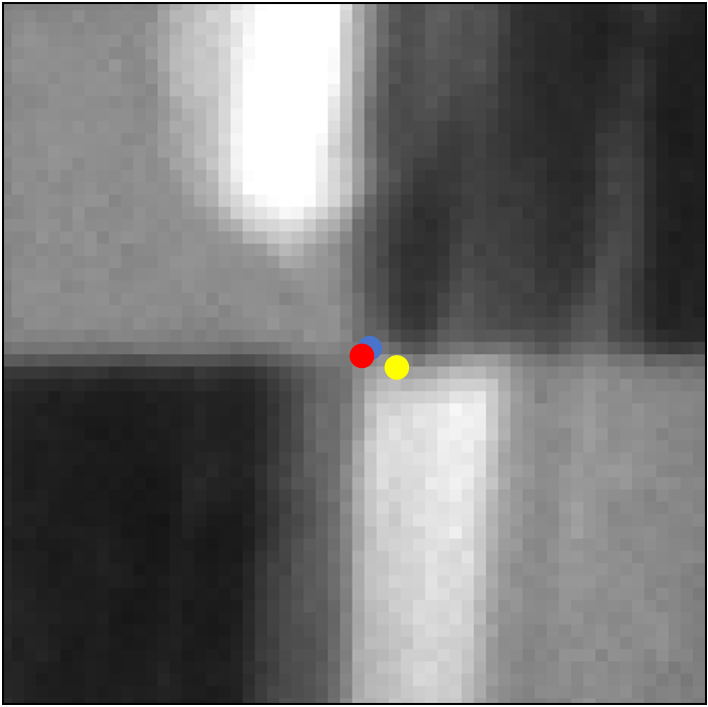
\includegraphics[width=\linewidth,height=1\textwidth]{images/5-1.png}
\end{minipage}
\hspace{0.2em}   % 调整缝隙，单位可用 em, cm, mm
\begin{minipage}{0.20\textwidth}
    \centering
    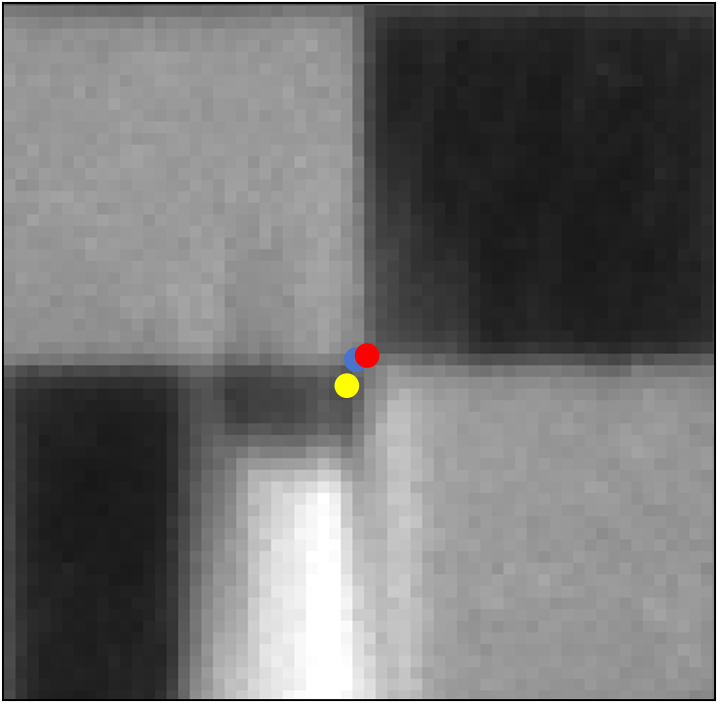
\includegraphics[width=\linewidth,height=1\textwidth]{images/5-2.png}
\end{minipage}
\hspace{0.2em}
\begin{minipage}{0.20\textwidth}
    \centering
    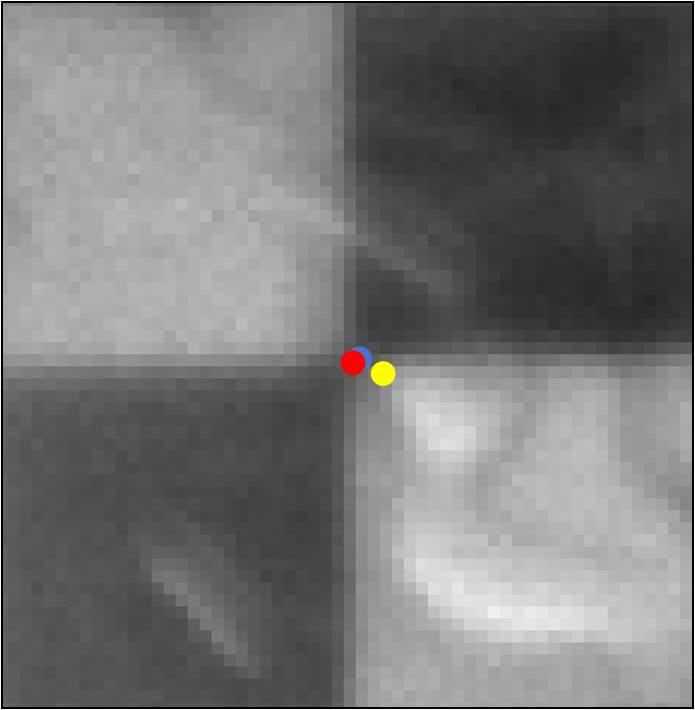
\includegraphics[width=\linewidth,height=1\textwidth]{images/5-3.png}
\end{minipage}
\hspace{0.2em}
\begin{minipage}{0.20\textwidth}
    \centering
    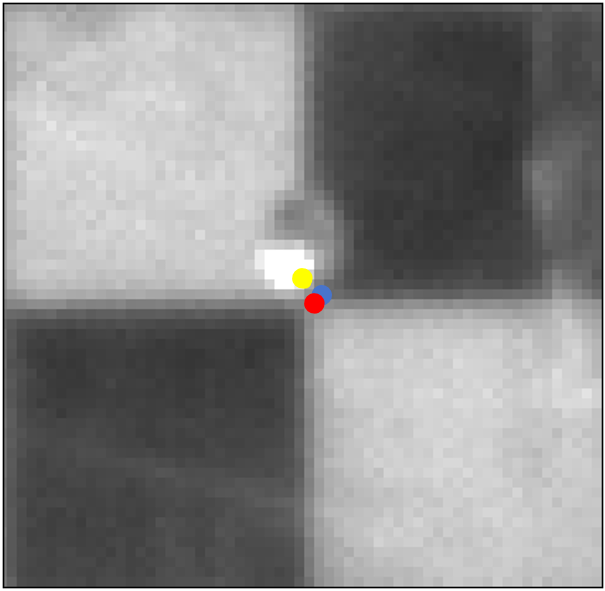
\includegraphics[width=\linewidth,height=1\textwidth]{images/5-4.png}
\end{minipage}

\caption{Comparison of Sub-pixel Corner Detection under Degradation. Ours (red points) and the Bouguet’s algorithm~\cite{bouguet2012camera} (yellow points) are compared, with blue points indicating the pixel-level corner coordinate inputs.}
\label{fig:comparison3}
\end{figure*}


\subsection{Multi-Chessboard Instance Detection}

In industrial scenarios, a single image may contain multiple chessboards with diverse scales, orientations, occlusions, and overlaps. To address this complexity, our method directly predicts semantic masks for chessboard regions, enabling one-shot separation of instances without predefined grid configurations. Connected-component analysis combined with heatmap-guided post-processing suppresses noise and splits weakly connected targets, ensuring accurate per-instance corner localization. This pipeline naturally supports parallel multi-instance processing and avoids reliance on row/column priors, yielding improved corner completeness and robustness under occlusion and clutter, as illustrated in Fig.~\ref{fig:multi_instance_ours}.




\begin{figure*}[htbp]
\centering
% 第一行
\begin{minipage}{0.24\textwidth}
    \centering
    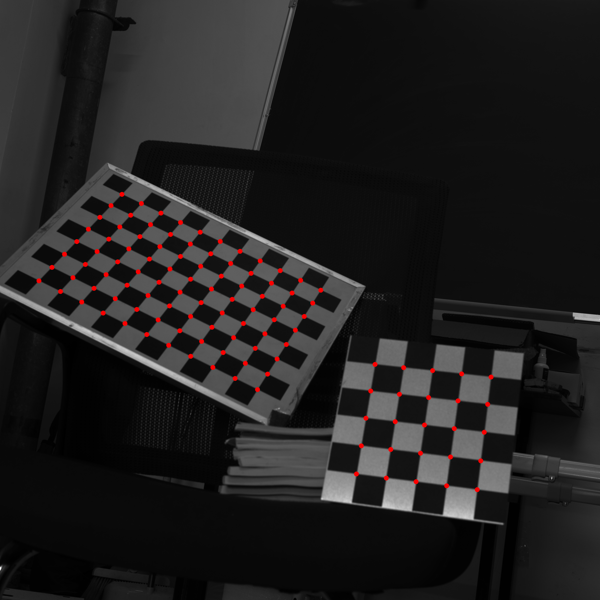
\includegraphics[width=\linewidth]{images/0-1.png}
    %\subcaption{(a)}
\end{minipage}
\begin{minipage}{0.24\textwidth}
    \centering
    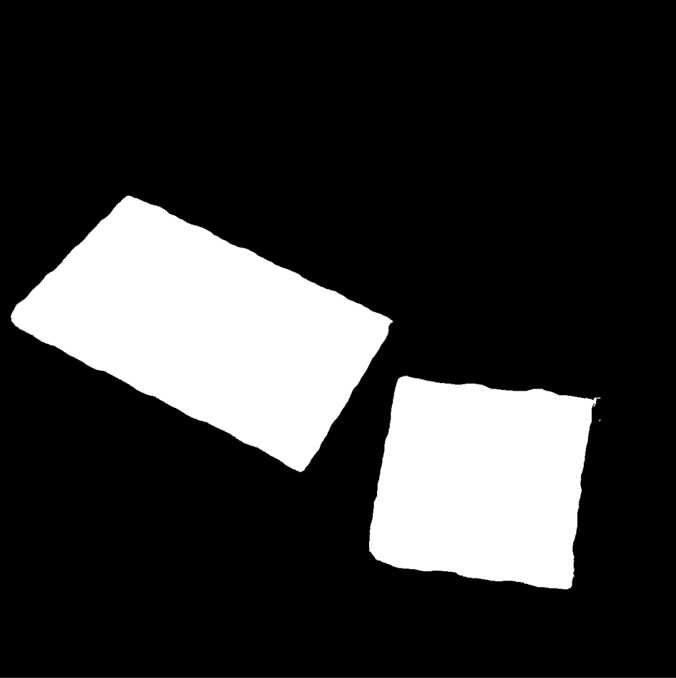
\includegraphics[width=\linewidth]{images/0-2.png}
    %\subcaption{(b)}
\end{minipage}
\begin{minipage}{0.24\textwidth}
    \centering
    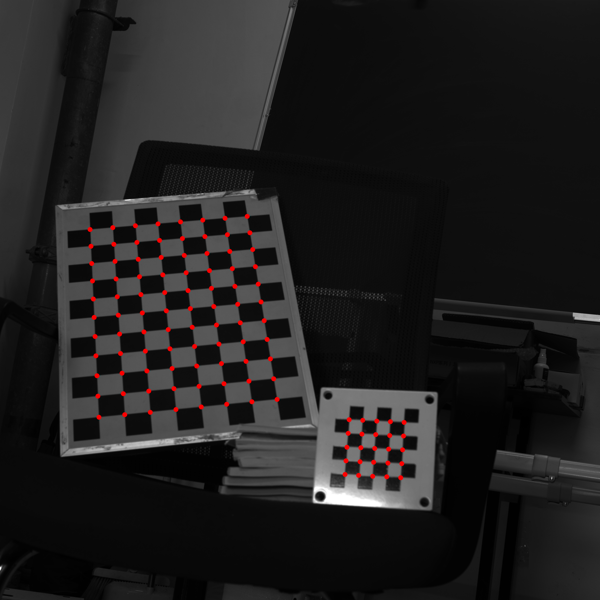
\includegraphics[width=\linewidth]{images/1-1.png}
    %\subcaption{(c)}
\end{minipage}
\begin{minipage}{0.24\textwidth}
    \centering
    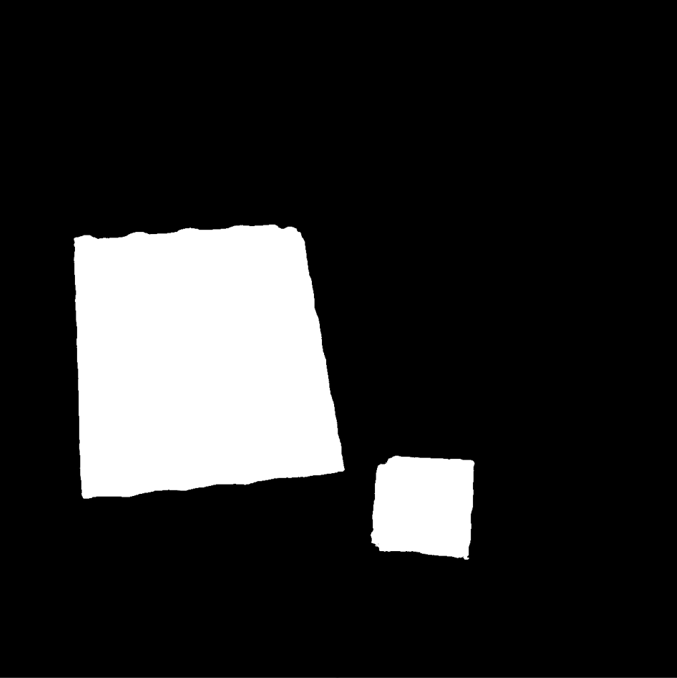
\includegraphics[width=\linewidth]{images/1-2.png}
    % \subcaption{(d)}
\end{minipage}

\vspace{0.5em} % 两行间距

% 第二行
\begin{minipage}{0.24\textwidth}
    \centering
    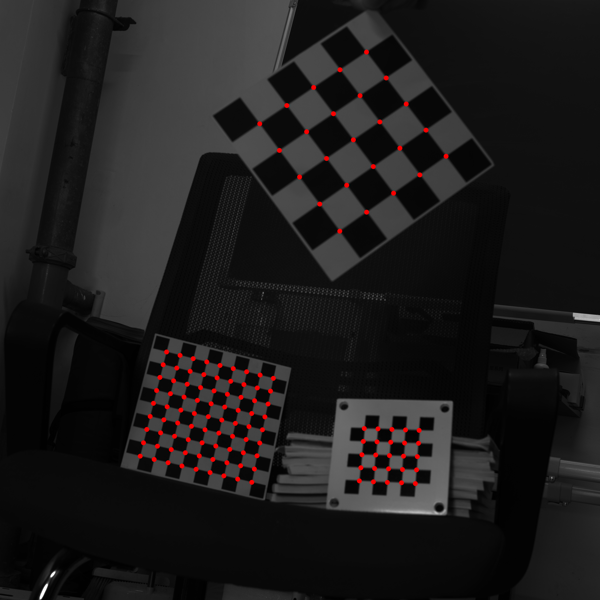
\includegraphics[width=\linewidth]{images/2-1.png}
    % \subcaption{(e)}
\end{minipage}
\begin{minipage}{0.24\textwidth}
    \centering
    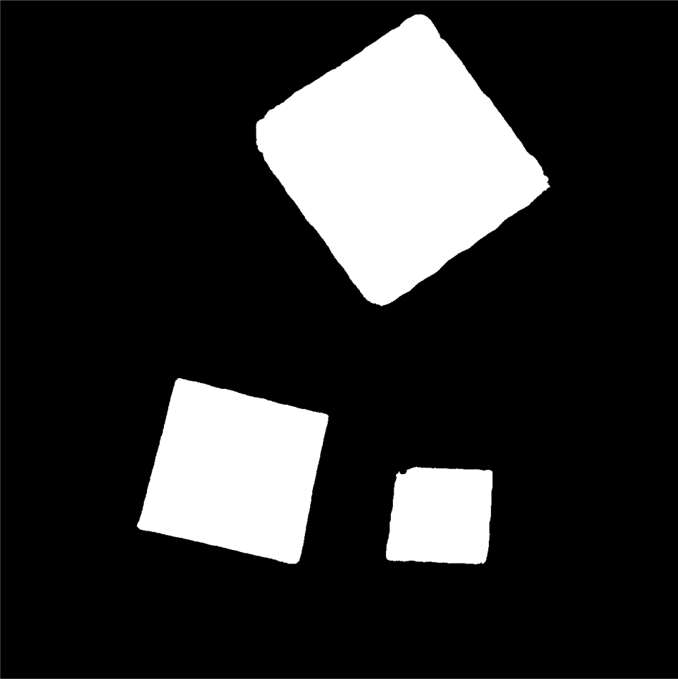
\includegraphics[width=\linewidth]{images/2-2.png}
    % \subcaption{(f)}
\end{minipage}
\begin{minipage}{0.24\textwidth}
    \centering
    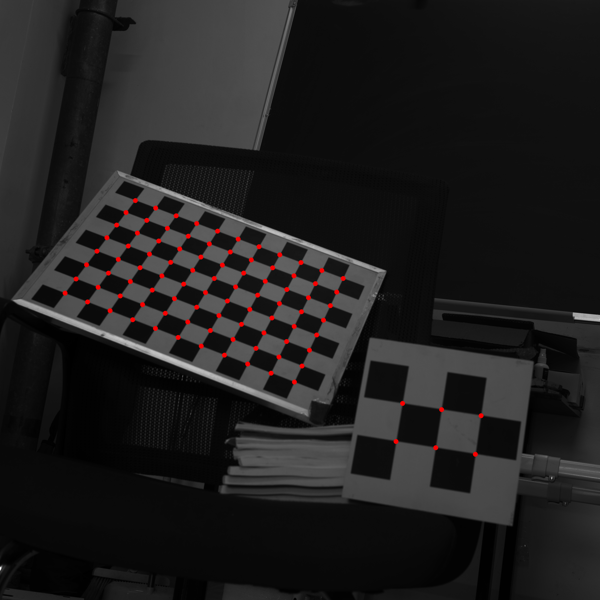
\includegraphics[width=\linewidth]{images/3-1.png}
    % \subcaption{(g)}
\end{minipage}
\begin{minipage}{0.24\textwidth}
    \centering
    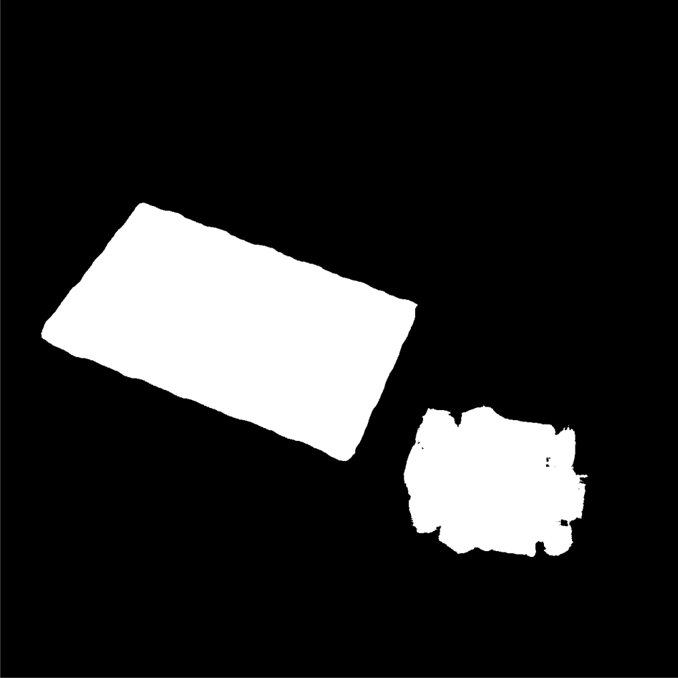
\includegraphics[width=\linewidth]{images/3-2.png}
    % \subcaption{(h)}
\end{minipage}

\caption{Representative qualitative results for multi-checkerboard scenes. 
Each subfigure shows detection results under varying conditions.}
\label{fig:multi_instance_ours}
\end{figure*}


\section{Conclusion}
In this work, we presented an improved UNet-based framework for accurate checkerboard corner detection, incorporating a dual-head structure for joint corner heatmap and region mask prediction and a sub-pixel refinement strategy for enhanced localization precision. experiments demonstrate that our method achieves state-of-the-art performance, particularly in noisy and challenging scenarios, while maintaining a favorable trade-off between accuracy and efficiency. Moreover, the proposed pipeline naturally extends to multi-checkerboard scenes through semantic masking and instance-level processing, enabling robust separation and precise localization of multiple, variably scaled checkerboards in a single forward pass. These capabilities make the method a compact, generalizable, and practical solution for real-world vision calibration tasks.

\nocite{*}
\bibliography{myReference}
\bibliographystyle{splncs04}

% \begin{thebibliography}{8}
% \bibitem{Harris1988}
% Harris C, Stephens M. A combined corner and edge detector[C]//Proceedings of the Fourth Alvey Vision Conference. 1988: 147-151.

% \bibitem{Kanade1974}
% Kanade T. Picture processing system by computer complex and recognition of human faces[D]. Kyoto University, 1974.

% \bibitem{Haralick1992}
% Haralick R M, Shapiro L G. Computer and robot vision[M]. Addison-Wesley Longman Publishing Co., Inc., 1991.

% \bibitem{Wang2002}
% Wang L L, Tsai W H. Camera calibration by vanishing lines for 3-D computer vision[J]. IEEE Transactions on Pattern Analysis and Machine Intelligence, 1991, 13(4): 370-376.

% \bibitem{Lucchese2001}
% Lucchese L, Mitra S K. Using saddle points for subpixel feature detection in camera calibration targets[C]//Asia-Pacific Conference on Circuits and Systems. IEEE, 2002, 2: 191-195.

% \bibitem{VanDeWeijer2006}
% Van De Weijer J, Gevers T, Smeulders A W M. Robust photometric invariant features from the color tensor[J]. IEEE Transactions on Image Processing, 2005, 15(1): 118-127.

% \bibitem{opencv_checkerboard}
% Bradski G, Kaehler A. Learning OpenCV: Computer vision with the OpenCV library[J]. Dr. Dobb's Journal of Software Tools, 2000, 2: 78-85.

% \bibitem{ocamcalib2006}
% Scaramuzza D, Martinelli A, Siegwart R. A toolbox for easily calibrating omnidirectional cameras[C]//2006 IEEE/RSJ International Conference on Intelligent Robots and Systems. IEEE, 2006: 5695-5701.

% \bibitem{bennett2014chess}
% Bennett S, Lasenby J. ChESS: Quick and robust detection of chess-board features[J]. Computer Vision and Image Understanding, 2014, 118: 197-210.

% \bibitem{hessian1999}
% Lindeberg T. Feature detection with automatic scale selection[J]. International Journal of Computer Vision, 1998, 30(2): 79-116.

% \bibitem{MATE2016}
% Donné S, De Vylder J, Goossens B, et al. MATE: Machine learning for adaptive calibration template detection[J]. Sensors, 2016, 16(11): 1858.

% \bibitem{spitschan2018robust}
% Spitschan B, Ostermann J. Robust Fourier-based checkerboard corner detection for camera calibration[C]//Iberoamerican Congress on Pattern Recognition. Springer, 2018: 538-546.

% \bibitem{Duda2018}
% Duda A, Frese U. Accurate detection and localization of checkerboard corners for calibration[C]//British Machine Vision Conference (BMVC). 2018: 1-12.

% \bibitem{ma2008robust}
% Awrangjeb M, Lu G. Robust image corner detection based on the chord-to-point distance accumulation technique[J]. IEEE Transactions on Multimedia, 2008, 10(6): 1059-1072.

% \bibitem{geiger2012automatic}
% Geiger A, Moosmann F, Car Ö, et al. Automatic camera and range sensor calibration using a single shot[C]//2012 IEEE International Conference on Robotics and Automation. IEEE, 2012: 3936-3943.

% \bibitem{wu2020checkerboard}
% Wu M, Wu J, Ma S, et al. Checkerboard corner detection based on corner gray distribution feature[J]. Laser Optoelectronics Progress, 2020, 57(10): 109-116.

% \bibitem{bouguet2012camera}
% Bouguet J Y. Camera calibration toolbox for MATLAB[EB/OL]. 2012. http://www.vision.caltech.edu/bouguetj/calib\_doc/index.html.

% \bibitem{salehi2017tversky}
% Salehi S S M, Erdogmus D, Gholipour A. Tversky loss function for image segmentation using 3D fully convolutional deep networks[J]. arXiv preprint arXiv:1706.05721, 2017.

% \bibitem{zhang2002flexible}
% Zhang Z. A flexible new technique for camera calibration[J]. IEEE Transactions on Pattern Analysis and Machine Intelligence, 2000, 22(11): 1330-1334.
% \end{thebibliography}
% \begin{thebibliography}{8}
% \bibitem{ref_lncs1}
% Yi K, Luo K, Luo X, et al. Ucmctrack: Multi-object tracking with uniform camera motion compensation[C]//Proceedings of the AAAI Conference on Artificial Intelligence. 2024, 38(7): 6702-6710.
% \end{thebibliography}
\end{document}
